%% Chapter 11 — LLM 서빙
\setcounter{chapter}{10}
\chapter{LLM 서빙}
\chaptersubtitle{자기회귀, KV 캐시, 연속 배치 — 엔진 안으로 들어간 운영체제}

\begin{calloutbox}{tbbblue}{tbbbluefill}
{\normalsize\bfseries\color{tbbblue}학습 목표}\par\vspace{3pt}
\begin{tbbitemize}
  \item 생성 트래픽에서 요청 수준 지연 시간 SLO가 의미를 잃는 이유를 설명하고, 두 가지 인간 상수(Miller 1968, 읽기 속도)를 예산으로 삼는 \textbf{두 시계} TTFT와 TPOT로 다시 작성한다.
  \item 한 번의 생성을 \textbf{프리필과 디코드}로 분해하고 각 단계의 산술 집약도를 계산한 뒤, 제10장의 루프라인으로 각 단계가 어떤 자원을 소진하는지 예측한다.
  \item 어텐션이 다시 읽는 값에서 \textbf{KV 캐시}를 도출하고 모델 카드로 크기를 계산한다. VRAM을 가중치, 런타임, 캐시 풀로 나누어 예산을 잡고 동시성을 메모리 수치로 표현한다.
  \item 프리필–디코드 간섭과 청크 프리필을 포함해 \textbf{연속 배치}(반복 수준 스케줄링)가 제9장의 깨진 가정을 어떻게 복구하는지 설명한다.
  \item \textbf{PagedAttention}을 어텐션에 이식한 가상 메모리로 이해하고, 블록 테이블, 공유, 쓰기 시 복사를 설명한다. 낭비를 회수한 결과 측정 처리량이 2–4×가 된 이유도 이해한다.
  \item \textbf{vLLM}을 운영한다. 제9장의 여섯 기관에 대응시키고, 메트릭을 읽고, 양자화한 AWQ 모델을 서빙하며, 동시 부하에서 TTFT/TPOT를 정직하게 측정한다. 이것이 실습이자 프로젝트의 새 SLO 문장이다.
\end{tbbitemize}
\end{calloutbox}

\vspace{2.5pt}

\begin{calloutbox}{tbbteal}{tbbtealfill}
{\normalsize\bfseries\color{tbbteal}핵심 용어}\par\vspace{3pt}
자기회귀 생성 · 프리필 대 디코드 · TTFT · TPOT / 초당 토큰 수(tokens-per-second) · 스트리밍(SSE) · 읽기 속도 하한 · KV 캐시 · GQA / MQA · KV 예산 · 입장 제어와 선점 · 연속 배치 · 반복 수준 스케줄링(Orca) · 프리필–디코드 간섭 · 청크 프리필 · PagedAttention · 블록 테이블 · 접두사 캐싱 · 쓰기 시 복사 · vLLM · 추측 디코딩 · 토큰 인식 부하 테스트
\end{calloutbox}

\vspace{2.5pt}

\begin{calloutbox}{tbblightgray}{tbbboxfill}
{\normalsize\bfseries\color{tbbink}장 구성}\par\vspace{3pt}
\textbf{11.1} 모델이 말을 걸다 — 대시보드는 거짓말한다    \textbf{11.2} 생성의 구조: 두 단계, 두 시계    \textbf{11.3} KV 캐시: 메모리가 새로운 동시성이다    \textbf{11.4} 연속 배치: 시내버스    \textbf{11.5} PagedAttention과 vLLM: 운영체제가 안으로 들어가다    \textbf{11.6} 실습: 실제 LLM 서빙, 스트리밍, 측정 — 이어서 요약, 연습문제, 더 읽을거리
\end{calloutbox}

\section{모델이 말을 걸다 — 대시보드는 거짓말한다}

지금까지 만든 모든 서빙 시스템에는 말하지 않은 가정 하나가 있었다. \textbf{요청 하나가 작업 단위다.} 분류 호출은 순방향 패스 한 번의 비용을 내고, 패스는 몇 밀리초가 걸리며, 그 수치의 백분위수를 약속하고 이에 맞게 프로비저닝한다. 제7장부터 제10장까지는 이 세계를 측정하고 최적화하며 가격을 매겼다. 지난주는 승리로 끝났다. TensorRT-INT8로 최적화한 3B 채팅 모델은 L4 한 대당 57 req/s에서 p99를 500 ms 아래로 유지했고, 약속대로 플릿 비용이 절반이 되었다. 그런데 월요일에 베타 사용자가 도착했다. 이들은 스윕에 넣어 둔 정형 프롬프트를 보내지 않았다. 자기소개서를 써 달라고 요청했다.

\begin{terminalbox}
\begin{Verbatim}[breaklines=true,breakanywhere=true,fontsize=\small,formatcom=\color{tbbtermfg},codes=\tbbcodeactive]
# monday 09:12. the Week-10 stack (INT8, 4 x L4), meeting REAL
# chat traffic for the first time. locust replays the beta logs:
$ locust -f chat_replay.py --headless -u 32 -r 4 --run-time 10m
 Type  Name     # reqs   # fails |  Avg     p50      p99   | req/s
 POST  /chat     4,102   0(0.0%) | 3,846   2,910   11,400  |  6.8
# p99 = 11.4 SECONDS against a 500 ms SLO. dashboard: solid red.
$ kubectl top pod -l app=chat      # surely something is dying?
NAME         CPU(cores)   MEMORY
chat-7f9b4   3210m        11.2Gi   # ...healthy.
$ nvidia-smi --query-gpu=utilization.gpu --format=csv,noheader
94 %                                # busy AND healthy.
# nothing is broken. the ANSWERS got long:
#   "reset my password?"        ->  40 tokens,   0.9 s
#   "write my cover letter..."  -> 700 tokens,  14.8 s
# the request stopped being a unit of work. the SLO measures noise.
\end{Verbatim}
\end{terminalbox}
\figcaption{사례 11-A  p99 폭발. 모든 구성 요소가 상태 검사를 통과하지만 SLO는 20배나 위반한다. 원인은 버그가 아니라 분포다. 응답 길이가 이제 100× 차이 나고 요청 지연 시간이 그 차이를 모두 물려받는다. 죽은 것은 시스템이 아니라 메트릭이다.}

이 사례의 낯섦을 잠시 곱씹어 보자. 이 책에서 처음 만나는 \textit{종류}의 실패다. 제7장의 용어로 보면 어떤 것도 회귀하지 않았다. 장치는 금요일과 똑같이 토큰마다 같은 작업을 수행한다. 깨진 것은 \textbf{계약의 단위}다. 이제 "요청" 하나에 필요한 작업은 40 tokens에서 4,000까지 세 자릿수 범위에 걸친다. 용량 계획이 아니라 \textit{사용자가 무엇을 묻고 모델이 어떻게 답하기로 하는지}가 양을 결정한다. 이 분포 위에서 요청 수준 p99를 약속하는 것은 날씨를 약속하는 것과 같다. 제10장의 최적화를 아무리 적용해도 해결되지 않는다. 토큰당 비용을 절반으로 줄여도 자기소개서는 7초가 걸린다. 평균은 아무도 설명하지 못했고, 이제 p99도 마찬가지다. 시스템 상태가 아니라 답변 길이를 추적하기 때문이다.

\subsection*{컴퓨팅에서 가장 오래된 인터페이스의 재발견}

해결책은 55년 간격을 두고 두 번 발견되었다. 이 책의 2주 차는 CP-67이 하나의 메인프레임을 여러 개로 나누는 시분할에서 시작했다. 지금 중요한 세부는 \textit{터미널이 무엇을 했는가}다. 터미널은 \textbf{답을 타이핑해 주었다.} 초당 10 characters 속도의 텔레타이프가 컴퓨터의 답을 스트림으로 전달하자 사용자들은 이를 좋아했다. 장치가 살아 있고 자신에게 집중하며 \textit{나를 위해 일하는 것}처럼 느껴졌다. 1968년 IBM의 Robert Miller는 이 감각 아래의 심리를 측정해 이후 모든 인터페이스 혁명에서도 살아남은 세 수치를 제시했다. \textbf{0.1 s} 아래에서는 즉각적으로 느껴지고, \textbf{1 s}까지는 사고의 흐름이 끊기지 않으며, \textbf{10 s}가 지나면 주의가 무너져 다른 작업으로 전환한다. 사람은 분당 약 250 words, 즉 초당 5–7 tokens를 읽는다는 인간 상수 하나를 더하면 대화형 AI의 전체 설계 공간이 이미 1968년의 종이 위에 그려진다.

이제 그 상수를 기준으로 사례 11-A를 다시 읽어 보자. 스트리밍하지 않은 자기소개서는 14.8 s 뒤에 도착해 Miller의 포기 구간 깊숙이 들어간다. 하지만 모델은 수백 밀리초 안에 \textit{첫 단어를 생성}했고, 나머지는 사람이 읽는 속도의 일곱 배인 \textasciitilde{}50 tokens/second로 만들었다. 같은 연산을 스트림으로 전달하면 1초의 흐름 구간 \textit{안쪽에 여유롭게} 들어오고 이후 영원히 독자보다 앞서간다. \textbf{스트리밍은 답을 더 빨리 만들지 않는다. 사용자가 경험하는 시계를 바꾼다.} 이것이 ChatGPT가 1억 명에게 선보인 진짜 혁신이다. 지연 시간 최적화가 아니라 계약의 재협상이었고, 이후 모든 채팅 제품이 1968년 텔레타이프처럼 답을 타이핑하는 이유다. §7.2는 이 모드에 이름을 붙이고 "11주 차"에 시계에 SLO를 부여하겠다고 약속했다. 이제 11주 차다.

\begin{tbbfigure}
  \adjustbox{max width=0.94\linewidth,max totalheight=0.46\textheight}{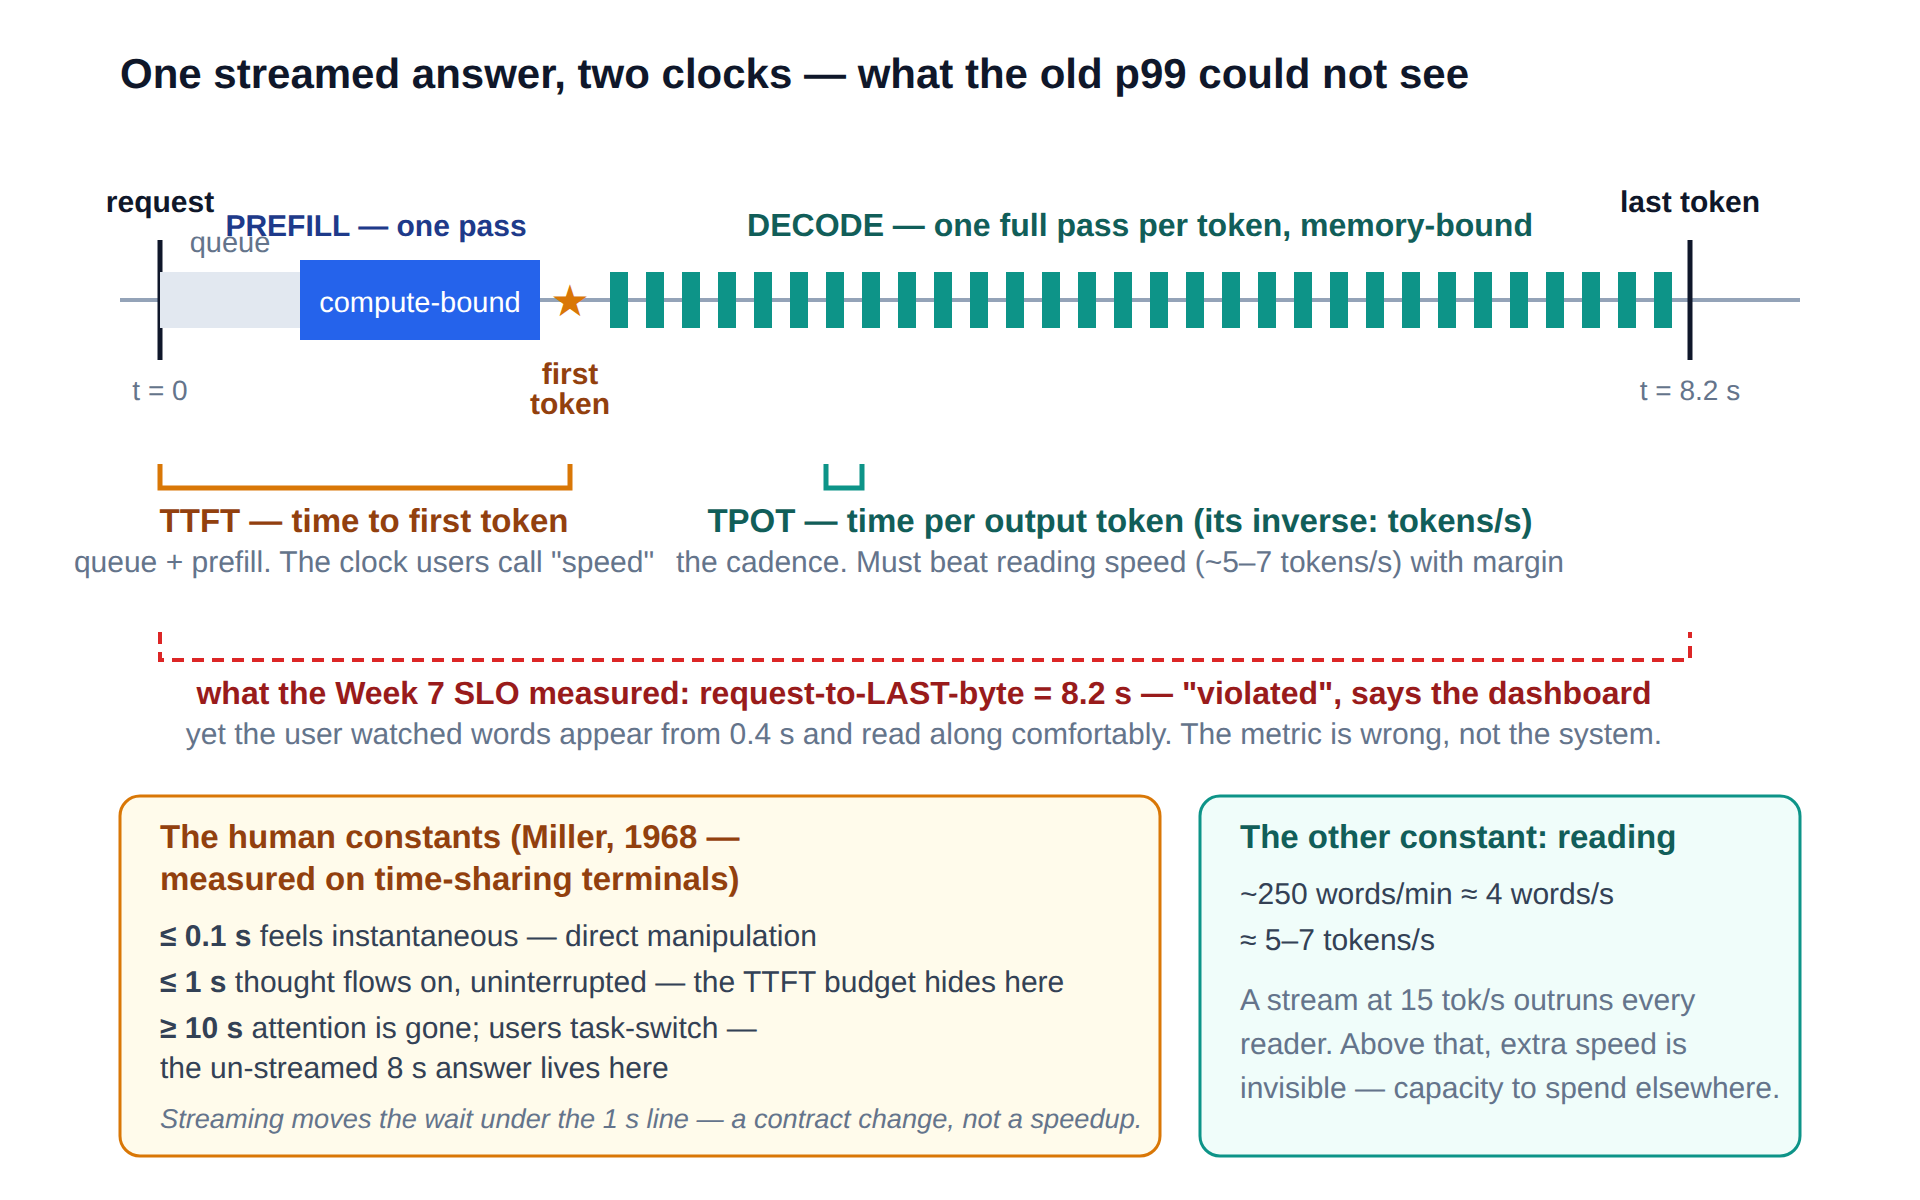
\includegraphics{figures/fig11-1_twoclocks.png}}\\[3pt]
  \figcaption{그림 11-1  하나의 스트리밍 답변과 두 시계. TTFT(대기열 + 프리필)는 "반응성이 있는가?"에 답하고, TPOT는 "읽는 속도보다 빠른가?"에 답한다. 기존의 요청부터 마지막 바이트까지 p99는 아무도 묻지 않은 질문에 답한다. Miller가 1968년에 제시한 임곗값과 읽기 속도가 예산이다.}
\end{tbbfigure}

따라서 프로젝트의 SLO 문장은 폐기하는 대신 다시 쓴다. 새 문장은 생각보다 관대하다. 기존 약속인 "p99 ≤ 500 ms"는 자신도 모르게 \textit{반응성}에 관한 약속이었다. 500 ms는 Miller의 1초 선 아래에 여유 있게 들어가므로 그대로 \textbf{TTFT 예산}이 된다. 여기에 \textbf{속도 조항}을 추가한다. 스트림당 tokens/second의 하한을 읽기 속도보다 넉넉히 높게 둔다. \textbf{용량 표현}도 바꾼다. 길이가 100× 차이 나는 환경에서 무의미한 초당 요청 수가 아니라 \textit{동시 스트림}을 쓴다. 실습에서 측정할 완전한 문장은 다음과 같다. \textbf{"TTFT p99 ≤ 500 ms, 스트림당 ≥ 15 tokens/s p50, 4-레플리카 L4 플릿에서 동시 스트림 100개, 월 \$900 이내."} 제7장 규율의 모든 조항인 백분위수, 임곗값, 부하, 비용은 살아남는다. 단위의 종만 바뀌었다.

\subsection*{두 번째 사례: 무언가가 기억하고 있다}

같은 날 오후, 이 장의 또 다른 수수께끼가 나타난다. 팀원이 수업을 위해 다중 턴 데모를 실행하면서 제2장에서 들인 습관대로 \code{nvidia-smi}를 계속 지켜본다. 모델은 6 GB다. 결과를 살펴보자.

\begin{terminalbox}
\begin{Verbatim}[breaklines=true,breakanywhere=true,fontsize=\small,formatcom=\color{tbbtermfg},codes=\tbbcodeactive]
# 14:00, demo day. multi-turn chat, ~30 slow-growing conversations.
$ watch -n 60 nvidia-smi --query-gpu=memory.used --format=csv,noheader
14:00    9,812 MiB    # weights (6 GB) + runtime + a few young chats
14:07   14,203 MiB    # ...the demo continues, nothing new deployed...
14:15   19,540 MiB    # no bigger model. no leak. no new users.
14:21   22,911 MiB    # the server is REMEMBERING something.
14:22   torch.cuda.OutOfMemoryError: CUDA out of memory. Tried to
        allocate 448.00 MiB (GPU 0; 23.99 GiB total capacity)
# exit 137's GPU cousin (Chs. 3/5) - and note the amount it wanted:
# 448 MiB. remember that number. §11.3 will compute it from scratch.
\end{Verbatim}
\end{terminalbox}
\figcaption{사례 11-B  서서히 증가하는 메모리. 가중치는 그대로인데 모든 대화의 토큰마다 메모리가 늘어난다. 결국 할당기가 정확히 448 MiB를 더 요구하다 실패한다. 누수는 없다. 모델은 열려 있는 모든 대화에 대해 계속 커지는 공책을 유지하지만, 아무도 그 공책의 예산을 잡지 않았다.}

두 사례와 두 수수께끼를 한 장에서 다룬다. 사례 A에서는 \textit{시간} 축이 깨졌다. 지연 시간을 토큰 단위로 다시 계약해야 한다. 사례 B에서는 \textit{메모리} 축이 깨졌다. 토큰마다 무언가가 자라며, 연산이 아니라 그것이 GPU에 몇 명의 사용자를 넣을 수 있는지 결정한다. 둘은 한 문장으로 정리할 수 있는 기계적 사실에서 비롯된다. \textbf{언어 모델은 출력 토큰마다 전체 순방향 패스를 한 번씩 실행하고 지금까지 생성한 모든 것을 참고해 답한다.} 그 루프가 §11.2다. 참고하는 공책은 §11.3이며, 448 MiB가 4,096토큰 대화 하나의 공책 크기와 메가바이트 단위까지 일치한다는 사실을 확인한다. GPU를 이런 루프로 가득 채우는 스케줄러는 §11.4, 공책의 선반 공간 낭비를 막는 메모리 관리자는 §11.5에서 다룬다. §11.6 실습에서는 vLLM, 초시계, 10달러어치 T4 시간을 사용해 이 모든 것을 직접 다룬다.

이 장은 책이 미뤄 둔 약속을 어느 장보다 많이 갚는다. 제1장은 KV 캐시를 "11주 차의 주인공"이라 부르고 Kwon 등의 논문을 "필독"으로 지정했다. 제6장에는 고정 세션의 결론과 정확히 60.0초에 끊기는 스트림이라는 빚이 있다. 제7장은 스트리밍에 SLO를 부여해야 한다. 제9장 상자 9-1의 작은 글씨, 즉 \textit{요청 형상이 비슷해야 한다}는 가정은 여기서 폭발하며 더 읽을거리에서는 "KV 캐시 강의 뒤"에 Orca를 보라고 안내했다. 제10장은 그룹별 INT4 용어의 실제 활용, 추측 디코딩 수단, AI ≈ 1인 matvec에 대한 답을 남겼다. 아래에서 모두 갚는다.

\begin{calloutbox}{tbbpurple}{tbbpurplefill}
{\normalsize\bfseries\color{tbbpurple}생각해 보기}\par\vspace{3pt}
\begin{tbbitemize}
  \item 사례 11-A의 서비스는 "모든 대시보드에서 정상"이지만 SLO를 20× 위반한다. 제5–9장에서 모두 녹색으로 나타날 대시보드 세 개와, 아직 어느 대시보드에도 없지만 실제로 사용자 불만을 예측하는 수치 하나를 제시하라. 그 수치는 기계적으로 어디에서 나오는가?
  \item Miller의 임곗값은 1968년 시분할 터미널에서 측정되었고 읽기 속도는 그보다도 오래된 상수다. "대화형 AI 제품 설계는 반세기 전에 생긴 상수로 과도하게 결정된다"는 주장에 찬성하거나 반박하라. LLM이 실제로 새로운 상수를 추가한다면 무엇인가?
  \item PM이 max\_tokens를 100으로 제한해 사례 11-A를 해결하자고 제안한다. "자기소개서는 더 이상 없다"는 뜻이다. 서빙 삼각형과 두 시계를 이용해 무엇을 포기하게 되고 어느 사용자가 이를 느끼는지 나열하라. 같은 자원을 나누는 방법 중 스트리밍이 엄격히 더 관대한 이유도 설명하라.
  \item 사례 11-B의 할당기는 448 MiB를 요구하다 실패했다. 다음 절을 읽지 않고 모델 카드에서 이 수치를 예측하려면 제1–10장에서 배운 어떤 양이 필요한지 모두 나열하고, 무엇이 커지는지 추측하라. §11.3에서 그 추측을 채점한다.
\end{tbbitemize}
\end{calloutbox}

\section{생성의 구조: 두 단계, 두 시계}

먼저 신비를 걷어 내자. 트랜스포머 언어 모델은 토큰 시퀀스를 읽고 \textbf{다음 토큰 하나의 확률 분포}를 출력하는 함수다. 할 수 있는 일은 이것뿐이다. 따라서 200토큰 답변을 만들려면 서빙 스택이 모델을 200번 실행해야 한다. 프롬프트를 넣고 토큰 \#1을 표본 추출한 뒤 이를 붙여 다시 실행하고 토큰 \#2를 뽑는다. 붙이고, 실행하고, 표본 추출하는 루프가 이어지며, 이를 \textbf{자기회귀(autoregressive) 생성}이라고 한다. 모델이 종료 토큰을 내거나 한도에 도달해야 끝난다. 두 시계, 증가하는 메모리, 깨진 배처, 이색적인 엔진 등 LLM 서빙의 낯선 모든 현상은 이 루프 하나와 이미 배운 루프라인에서 나온다. 제10장의 도구로 요청 하나를 분해해 보자.

\begin{tbbfigure}
  \adjustbox{max width=0.94\linewidth,max totalheight=0.46\textheight}{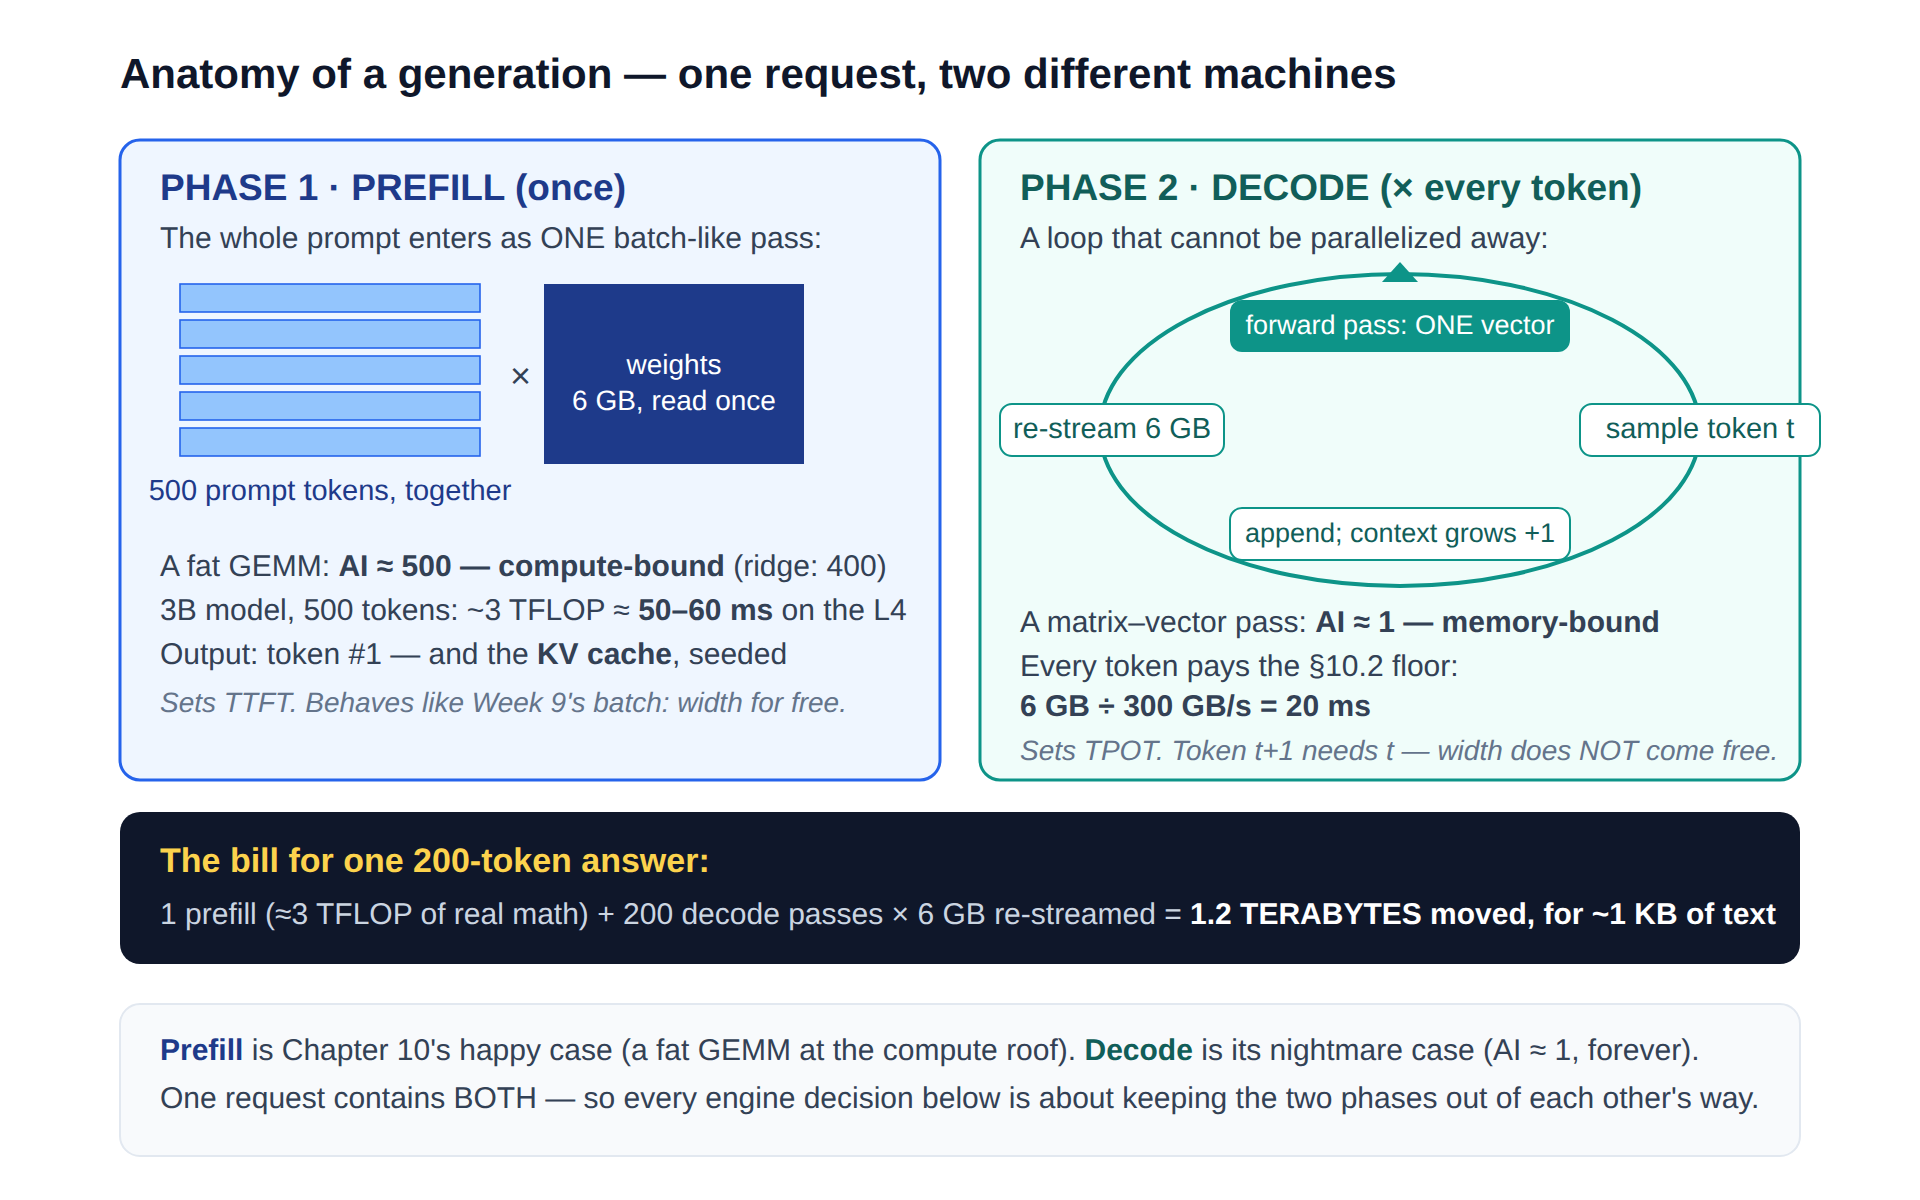
\includegraphics{figures/fig11-2_autoregress.png}}\\[3pt]
  \figcaption{그림 11-2  요청 하나와 두 장치. 프리필은 한 번의 연산 병목 패스로 프롬프트 전체를 처리해 캐시를 채운다. 이후 디코드는 토큰마다 전체 순방향 패스를 실행하며 모든 가중치를 다시 스트리밍하므로 영원히 메모리 병목인 루프를 돈다. 엔진의 역할은 두 단계가 서로 방해하지 않게 하는 것이다.}
\end{tbbfigure}

\subsection*{프리필: 이미 알고 있는 큰 GEMM}

첫 패스는 특별하다. 프롬프트의 모든 토큰은 이미 \textit{알려져} 있어 그 사이에서 표본 추출할 필요가 없다. 따라서 모델은 500개 토큰을 \textbf{한 번의 패스에서 함께} 처리한다. 서로에게 어텐션하는 500개 항목을 9주 차 배치로 묶은 것과 같다. 제10장의 세 수치로 보면 이는 큰 GEMM이다. 산술 집약도 ≈ 토큰 수다. 스트리밍한 가중치마다 500토큰 분량의 작업을 수행하므로 500토큰 패스는 L4의 \textasciitilde{}400 능선 \textit{위}에 놓여 실제로 \textbf{연산 병목}이다. 루프라인에서 가장 좋은 영역이다. 비용은 정직한 작업에서 나온다. \textasciitilde{}2 FLOPs per parameter per token × 3B × 500 ≈ \textbf{3 TFLOP}이며, 현실적인 효율에서 L4가 50–60 ms 동안 처리한다. 프리필(prefill)은 두 가지를 만든다. 첫째는 \textbf{첫 출력 토큰}이므로 프리필 시간이 TTFT의 거의 전부다. 둘째는 앞의 두 사례에서 이름을 기다려 온 부산물이다. 모든 프롬프트 토큰의 K와 V 텐서를 만들어 이후 루프를 위해 캐시한다(§11.3).

\subsection*{디코드: 끝나지 않는 matvec}

이어서 루프가 시작되면 장치의 종이 바뀐다. 각 디코드 단계는 방금 표본 추출한 \textbf{토큰 하나}를 전체 네트워크에 넣어 다음 분포를 얻는다. 토큰 하나는 처음부터 끝까지 행렬–\textit{벡터} 연산을 뜻한다. 제10장 첫 워크로드였던 AI ≈ 1, 즉 연산을 곁들인 바이트 배달 서비스다. 단계마다 \textasciitilde{}6 GFLOP을 수행하기 위해 6 GB의 가중치 전체를 다시 스트리밍하므로 §10.2의 하한인 \textbf{6 GB ÷ 300 GB/s = 20 ms}를 매번 부담한다. 여기에 실행과 표본 추출에 1–2밀리초가 더해진다. 한 \textit{시퀀스 안에서는} 단계가 중첩될 수 없다. token t+1의 입력이 바로 token t이므로 루프는 본질적으로 직렬이다. 배치도 컴파일러도 어떤 묘수도 이 의존성을 없애지 못한다. §11.5의 추측 디코딩만 조금 휘게 한다. 디코드가 TPOT를 결정하고 TPOT는 메모리 벽에 고정된다. 제10장이 배치 1 생성을 거듭 "가장 가혹한 모습의 벽"이라 부른 이유다.

\begin{terminalbox}
\begin{Verbatim}[breaklines=true,breakanywhere=true,fontsize=\small,formatcom=\color{tbbtermfg},codes=\tbbcodeactive]
# one instrumented request against a single unloaded L4 replica:
$ python two_clocks.py --url http://chat-l4:8000 --prompt 500tok.txt
tokenize + queue + prefill (500 tok):     73.8 ms   <- TTFT
decode: 200 tokens in 4.28 s:             21.5 ms/token  (46.5 tok/s)

# sanity, against §10.2 (no profiler, as always):
#   decode floor: 6 GB / 300 GB/s        = 20.0 ms  -> observed 21.5
#   overhead: launches+sampling+attention =  1.5 ms  -> a small a
#   prefill: 3 TFLOP / (~55 TFLOPS eff.) = ~55 ms   -> observed ~65
# prefill did 500 tokens of work in ~3.4 decode-tokens' time.
# two machines, one API. every engine decision follows from this.
\end{Verbatim}
\end{terminalbox}
\figcaption{터미널 기록 11-1  두 시계를 측정하고 제10장의 하한과 맞춘 결과. 프리필은 연산이며 디코드 약 3.4단계의 비용으로 500 tokens를 처리한다. 디코드는 대역폭이며 20 ms 하한에 소량이 더해진다. TTFT ≈ 대기열 + 프리필, TPOT ≈ 하한이다.}

\subsection*{두 시계에 SLO를 부여하다 — 스트림에 돌아온 Little의 법칙}

이제 §11.1의 계약을 선언하는 데 그치지 않고 설계할 수 있다. \textbf{TTFT}는 대기열 + 토큰화 + 프리필이다. 하한은 프리필 연산이며 500토큰 프롬프트에서 \textasciitilde{}65 ms다. 따라서 500 ms 예산 중 \textasciitilde{}430 ms를 대기열 처리에 쓸 수 있다. 배치 입장 제어(§11.4)에 실제로 사용할 수 있는 예산이며, 부하가 TPOT보다 TTFT를 먼저 무너뜨리는 이유다. \textbf{TPOT}는 디코드 하한에 스케줄러가 더하는 비용을 합친 값이다. 부하가 없을 때 21.5 ms (46 tok/s)이고 동시 스트림이 대역폭을 나눌수록 점진적으로 나빠진다. §11.3에서 정확히 계산한다. \textbf{종단 간 시간}도 여전히 존재한다. 200토큰 답변은 73.8 ms + 199 × 21.5 ms ≈ \textbf{4.4 s} 뒤에 도착한다. 하지만 이제 답변 길이가 지배하는 \textit{파생} 수치로서 보고는 하되 약속하지 않는다. 스트림이 주는 이점도 보자. 독자가 200토큰을 읽는 데 \textasciitilde{}30초가 걸리지만 시스템은 4.4초 만에 전달한다. 스트림은 이를 읽는 눈보다 일곱 배 앞서간다.

용량 계획도 익숙한 법칙을 통해 살아남는다. 제7장의 \textbf{L = λW}는 "고객"이 무엇인지 개의치 않으므로 다시 정의하면 된다. \textit{스트림} 하나가 W ≈ TTFT + N·TPOT초 동안 좌석을 점유한다. 200토큰 답변에서 W ≈ 4.4 s다. 동시 스트림 32개를 수용하는 레플리카가 정상 상태에서 받아들일 수 있는 도착률은 λ = 32 ÷ 4.4 ≈ \textbf{7.3 requests/s}다. 32가 어디에서 나오는지는 §11.3에서 설명한다. 이를 사례 11-A와 비교해 보자. 실패한 플릿은 사용률이 고정된 상태에서 6.8 req/s로 측정되었다. 모든 것이 "깨진" 날에도 법칙은 잡음 범위 안에서 들어맞았다. 제2장의 플릿 크기를 정한 공식이 여기서도 통한다. W의 의미만 달라졌다.

\begin{calloutbox}{tbbpurple}{tbbpurplefill}
{\normalsize\bfseries\color{tbbpurple}생각해 보기}\par\vspace{3pt}
\begin{tbbitemize}
  \item 터미널 기록 11-1의 프리필은 디코드 3.4토큰 시간에 500토큰 분량의 작업을 했다. L4의 121 TFLOPS를 기준으로 각 단계의 유효 FLOP 사용률을 계산하라. 루프라인 용어로 디코드의 나머지 \textasciitilde{}97\% 연산 용량이 어디로 갔는지 설명하라.
  \item 한 팀원은 "프롬프트를 줄여 TTFT를 낮추자"고 하고 다른 팀원은 "디코드보다 프리필을 먼저 받아 TTFT를 낮추자"고 한다. 각 제안은 누구의 어느 시계에 비용을 부과하는가? 두 번째 제안을 정식화하는 §11.4의 메커니즘은 무엇인가?
  \item 제10장에서 배포한 INT8 변형(3 GB 가중치, 같은 GPU)을 대상으로 터미널 기록 11-1을 다시 계산하라. 어느 시계가 얼마나 개선되며, 다른 시계는 왜 거의 움직이지 않는가? 힌트: 프리필은 연산 병목이다.
  \item L = λW로 전체 플릿을 계산하라. 동시 스트림 100개가 필요하고 W ≈ 4.4 s다. 제품이 감당할 수 있는 도착률은 얼마인가? 이제 평균 답변 길이를 두 배로 늘려라. 세 SLO 조항 중 무엇이 먼저 깨지며, 이를 해결하려면 무엇을 구매해야 하는가?
\end{tbbitemize}
\end{calloutbox}

\section{KV 캐시: 메모리가 새로운 동시성이다}

사례 11-B의 서버는 "무언가를 기억"하고 있었다. 이제 그 정체를 알아보자. 모든 트랜스포머 계층 안에서 어텐션(attention)은 현재 토큰이 이전의 모든 토큰을 참고하게 한다. 기계적으로 현재 토큰의 \textit{쿼리} 벡터를 각 과거 토큰의 \textbf{키} 벡터와 비교하고 그 \textbf{값} 벡터를 섞는다. 각 토큰이 위치에 고정되고 나면 K와 V 벡터는 그 토큰의 결정론적 함수가 되므로 두 선택지가 생긴다. 매 단계 \textbf{다시 계산}하면 t단계에서 이미 알던 값을 다시 얻기 위해 이전 t−1개 토큰 전체를 모든 계층에 다시 통과시켜야 한다. 대화 중간쯤에는 새 토큰마다 프리필 한 번의 비용이 들고, 2,000토큰 대화는 약 \textit{200만 번}의 불필요한 토큰-계층 연산을 수행한다. 아니면 \textbf{캐시}할 수 있다. 각 토큰의 K와 V를 정확히 한 번 계산해 저장하고 이후 모든 단계가 VRAM에서 읽게 한다. 세상의 모든 서빙 스택은 캐시를 택한다. 루프의 토큰당 연산은 일정해지는 대신 대화가 살아 있는 동안 토큰마다, 계층마다 K,V 행 하나씩 메모리가 늘어난다. 사례에서 본 점진적 증가가 이것이다.

\subsection*{모델 카드에서 크기 계산하기 — 속설은 필요 없다}

토큰당 비용은 아키텍처에서 바로 읽을 수 있다. 책의 3B 모델은 28개 계층을 갖고, 거의 모든 현대 LLM처럼 \textbf{그룹 쿼리 어텐션(GQA)}을 사용한다. 쿼리 헤드 24개가 각각 128차원인 KV 헤드 8개를 \textit{공유}한다. 연산이 아니라 캐시를 3× 줄이기 위한 구조다. 계층마다 토큰 하나에 8 × 128개 값의 K 벡터 하나와 V 벡터 하나를 저장한다. FP16에서는 2 × 28 × 8 × 128 × 2 bytes = \textbf{114,688 bytes ≈ 112 KB per token}이다. 따라서 4,096토큰 대화는 4,096 × 114,688 bytes = \textbf{469,762,048 bytes = 448.00 MiB}를 차지한다. 사례 11-B에서 요청하다 실패한 할당량과 바이트 단위까지 일치한다. 수수께끼의 원인은 누수가 아니었다. 대화 30개가 아무도 예산을 잡지 않은 정당한 메모리를 각각 최대 0.5기가바이트씩 들고, 한 번에 112 KB 행 하나만큼 자라고 있었다.

\begin{terminalbox}
\begin{Verbatim}[breaklines=true,breakanywhere=true,fontsize=\small,formatcom=\color{tbbtermfg},codes=\tbbcodeactive]
$ python kv_math.py --layers 28 --kv-heads 8 --head-dim 128 --dtype fp16
per token:            2 x 28 x 8 x 128 x 2 B = 114,688 B  (112 KB)
per 4k conversation:  4096 x 112 KB           = 448.00 MiB   # !!

# now budget the L4 (24 GB), vLLM-style at 90% utilization:
  usable            24.0 x 0.90 = 21.6 GB
  weights (FP16)                -  6.0 GB   # resident forever
  activations + CUDA + runtime  -  2.5 GB
  KV pool                       = 13.1 GB  -> ~115,000 tokens
# = 28 conversations at 4k. or 115 at 1k. THAT is your concurrency.
# note what is NOT in this arithmetic: FLOPS. compute stopped being
# the binding resource the moment the model started talking back.
\end{Verbatim}
\end{terminalbox}
\figcaption{터미널 기록 11-2  모델 카드에서 계산한 캐시. 사례 11-B의 448 MiB를 관찰이 아니라 도출했다. L4의 좌석 수는 13 GB 풀을 토큰당 112 KB로 나누는 문제다. 동시성이 메모리 수치가 되었다.}

\begin{tbbfigure}
  \adjustbox{max width=0.94\linewidth,max totalheight=0.46\textheight}{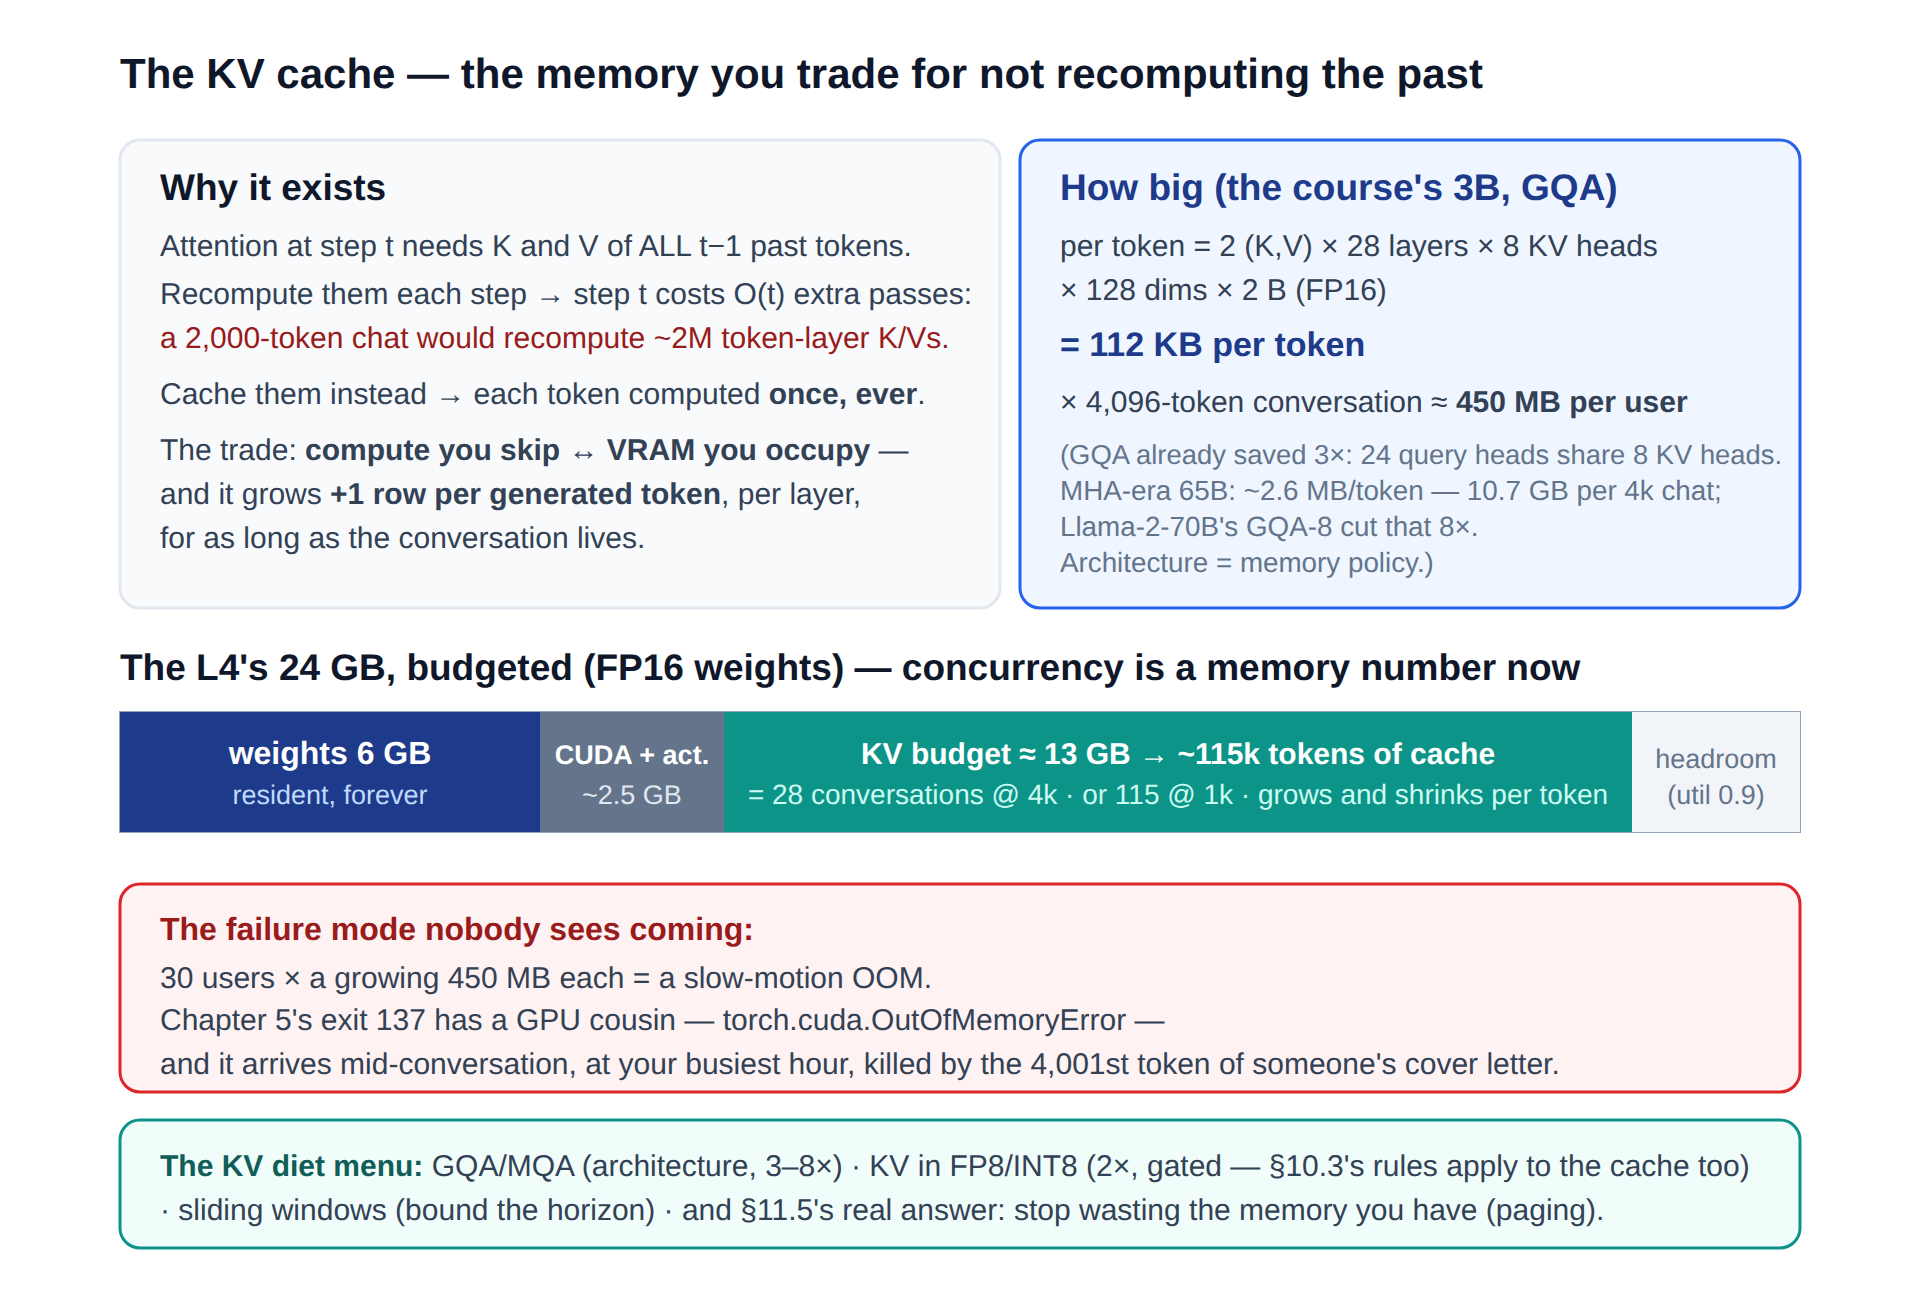
\includegraphics{figures/fig11-3_kvcache.png}}\\[3pt]
  \figcaption{그림 11-3  캐시가 존재하는 이유와 토큰당 비용, L4의 24 GB를 가중치, 런타임, KV 풀로 나눈 예산. GQA가 이미 비용을 3× 줄였고 다른 경량화 기법이 더 줄인다. §11.5는 남은 공간의 낭비를 막는다.}
\end{tbbfigure}

\subsection*{캐시가 디코드 단계에 미치는 영향 — 증가하는 b}

캐시는 점유 공간일 뿐 아니라 \textbf{트래픽}이다. 어텐션이 과거 전체를 참고하므로 각 디코드 단계는 시퀀스가 보유한 캐시의 모든 K,V를 \textit{읽어야} 한다. 한 단계의 바이트는 가중치 + 배치의 전체 캐시다. 제9장의 법칙을 조금 바꾸어 \textbf{t(step) ≈ (W\_bytes + Σ KV\_bytes(context)) ÷ bandwidth}라고 쓰자. 평균 컨텍스트가 4k인 배치 32에서 책의 모델을 실행하면 bytes = 6 GB + 32 × 0.47 GB ≈ \textbf{21 GB per step → \textasciitilde{}70 ms → \textasciitilde{}14 tokens/s per stream, \textasciitilde{}460 tokens/s aggregate}다. 배치 1의 6.47 GB → 21.5 ms → 46 tok/s와 비교해 보자. 제9장의 거래를 스트림에 맞게 다시 표현하면 \textbf{스트림당 지연 시간을 3× 늘리는 대신 집계 처리량을 10× 얻는 것}이다. 모든 스트림은 여전히 읽기 속도보다 빠르다. 새 항의 동작에 주목하자. 가중치는 같은 6 GB로 모두를 처리해 배치 전체에 상각된다. 이는 9주 차의 a다. 반면 \textbf{KV 바이트는 배치에 따라 증가}한다. 각 스트림이 자체 과거를 끌고 오므로 컨텍스트와 함께 커지는 b다. n × 0.47 = 6으로 놓으면 교차점을 찾을 수 있다. \textbf{동시 4k 대화가 \textasciitilde{}13개를 넘으면 캐시가 모델보다 무겁다.} 규모가 커지면 LLM 서버는 답을 만드는 네트워크보다 대화를 읽는 데 더 많은 대역폭을 쓴다.

이 계산 하나가 현대 LLM 서빙 연구 과제의 절반을 조용히 설명하므로 그 귀결을 더 살펴보자. \textit{긴 컨텍스트는 모두에게 부과되는 세금}이다. 32k-token 문서 대화 하나는 \textbf{모든 단계에서} 3.8 GB의 캐시를 벽 너머로 끌고 가 함께 배치된 모든 스트림을 늦춘다. 길이 제한과 컨텍스트 가격 책정은 인색함이 아니라 물리학이다. \textit{캐시 때문에 GQA/MQA가 존재한다.} Shazeer는 2019년 MHA의 많은 KV 헤드가 추론에서 무엇을 사는지 묻고 "대부분 바이트"라고 답했다. \textit{KV 캐시 양자화}가 표준 수단인 이유도 같다. FP8은 112 KB를 절반으로 줄이며, §10.3의 게이트는 가중치와 똑같이 캐시에 적용된다. \textit{슬라이딩 윈도 모델}이 과거 범위를 아예 제한하는 이유도 여기에 있다. 입장 문제도 더 까다로워진다. 새 스트림은 \textbf{예측할 수 없이 커질} 풀 공간을 필요로 한다. 풀이 가득 차면 엔진은 입장을 대기열에 두거나 실행 중 스트림을 \textbf{선점(preemption)}해야 한다. 블록을 퇴거시키고 나중에 다시 프리필하여 메모리를 되찾는 대신 연산 비용을 낸다. 대기, 선점, 거부 중 \textit{무엇을} 고를지가 스케줄링이며 §11.4의 주제다.

\subsection*{다중 턴 채팅: 캐시와 상태 비저장 웹의 만남}

배처로 넘어가기 전에 제6장의 빚을 갚는 귀결 하나를 더 살펴보자. HTTP API는 상태를 저장하지 않으므로 대화의 각 턴이 \textbf{전체 기록}을 프롬프트로 다시 보낸다. 기계적으로 서버가 매 턴 전체 대화를 다시 \textit{프리필}한다는 뜻이다. 3,000토큰 대화의 5번째 턴은 4턴 전에 똑같이 계산한 K,V 행을 다시 만들기 위해 3,000토큰 프리필 비용, 즉 순수 연산 \textasciitilde{}350 ms를 낸다. 누군가 보관해 두지 않았다면 그렇다. 이를 보관하는 방식을 \textbf{접두사 캐싱(prefix caching)}이라 하며 §11.5의 블록 메커니즘은 거의 공짜로 만든다. 하지만 제6장의 고정 세션 긴장을 정확히 되살린다. 보관한 행은 \textbf{한 레플리카의 VRAM}에 있으므로 5번째 턴을 다른 레플리카로 라우팅하면 조용히 전체 프리필 비용을 다시 낸다. 이 긴장을 기억해 두자. §11.5에서는 어피니티를 정확성 요구사항이 아닌 \textit{성능 힌트}로만 취급하는 성숙한 방식으로 해결한다. 아래 생각해 볼 문제에서 먼저 양쪽 비용을 계산한다.

\begin{calloutbox}{tbbpurple}{tbbpurplefill}
{\normalsize\bfseries\color{tbbpurple}생각해 보기}\par\vspace{3pt}
\begin{tbbitemize}
  \item 사례 11-B의 시간선을 정량적으로 재구성하라. 24 GB 카드에서 9.8 GB를 바닥으로 삼고 대화 \textasciitilde{}30개가 각각 \textasciitilde{}2 tokens/s씩 자란다. 실패할 시각을 예측한 뒤 실제 곡선이 더 울퉁불퉁한 이유를 설명하라. 힌트: 답변은 끝나고 사용자는 멈추며 새 입장이 도착한다.
  \item PM은 "모델이 지원하니까" 128k 컨텍스트 요금제를 원한다. 책의 3B 모델에서 128k 대화 하나가 차지하는 KV 바이트, 배치 8의 단계별 트래픽, 퇴거되는 좌석 수로 비용을 계산하라. 이어 요금제의 가격 구조와 입장 규칙을 제안하라.
  \item 터미널 기록 11-2의 좌석 수를 (a) 제10장에서 배포한 INT8 가중치, (b) 여기에 FP8 KV 캐시 추가, (c) 둘에 GQA→MQA(KV 헤드 1개)까지 적용한 경우에 대해 다시 계산하라. 어느 단일 변경이 가장 많은 좌석을 사며, 무엇에 §10.3의 게이트가 가장 시급한가?
  \item 단계 비용 모델에 따르면 32k 문서 대화 하나를 짧은 대화 31개와 함께 배치하면 모두 느려진다. 큰 대화가 있을 때와 없을 때 각 스트림의 TPOT를 계산한 뒤 실제로 배포할 공정성 정책을 설계하라. 좌석별 KV 할당량, 별도 풀, 가격 책정을 고려할 수 있다.
  \item 제3장은 페이지 캐시를 "회수 가능한 짐", 익명 메모리를 "필수 메모리"라고 설명했다. KV 캐시는 어느 쪽인가? 답을 바탕으로 메모리 압박에서 엔진이 웹 서버에는 불가능했던 어떤 작업을 할 수 있는지 설명하라. §11.4의 선점이 그 결론이다.
\end{tbbitemize}
\end{calloutbox}

\section{연속 배치: 시내버스}

배치는 여전히 경제성의 전부다. §11.3의 계산에서 스트림 하나는 가중치 스트림 가치의 \textasciitilde{}97\%를 쓰지 못하지만 동승자 30명이 이를 회수했다. 그렇다면 9주 차의 동적 배처로 생성 요청을 모으면 될 것 같지만, 작은 글씨의 조항 하나 때문에 실패한다. 상자 9-1은 동적 배치가 \textbf{형상이 비슷한 요청}을 가정한다고 경고했다. 제10장의 규칙 ③은 \textit{입력}의 제각각인 길이에 패딩 비용을 부과하고 버킷팅을 제시했다. 생성은 버킷팅으로 해결할 수 없는 문제를 만든다. \textbf{출력 길이가 제각각이고 미리 알 수도 없다.} 요청 네 개가 함께 들어와 배치가 공유 디코드 루프를 돈다. 하나는 token 32에, 다른 하나는 210에 끝난다. \textit{정적} 배치에서는 일찍 끝난 요청의 좌석이 가장 긴 승객이 끝날 때까지 \textbf{죽은 채} 따라다닌다. 빈 좌석으로 가득한 버스 밖에는 새 요청이 줄을 선다. 수치는 명확하다. 답변 길이가 10–100× 차이 나면 좌석-단계 사용률은 약 50\%에 그친다. 더 가혹하게도 새 요청의 TTFT에는 먼저 탄 사람이 쓰고 있는 \textit{남은 글 전체}가 포함된다. 사례 11-A의 11.4초 p99에는 또 하나의 원인이 있었다.

\begin{tbbfigure}
  \adjustbox{max width=0.94\linewidth,max totalheight=0.46\textheight}{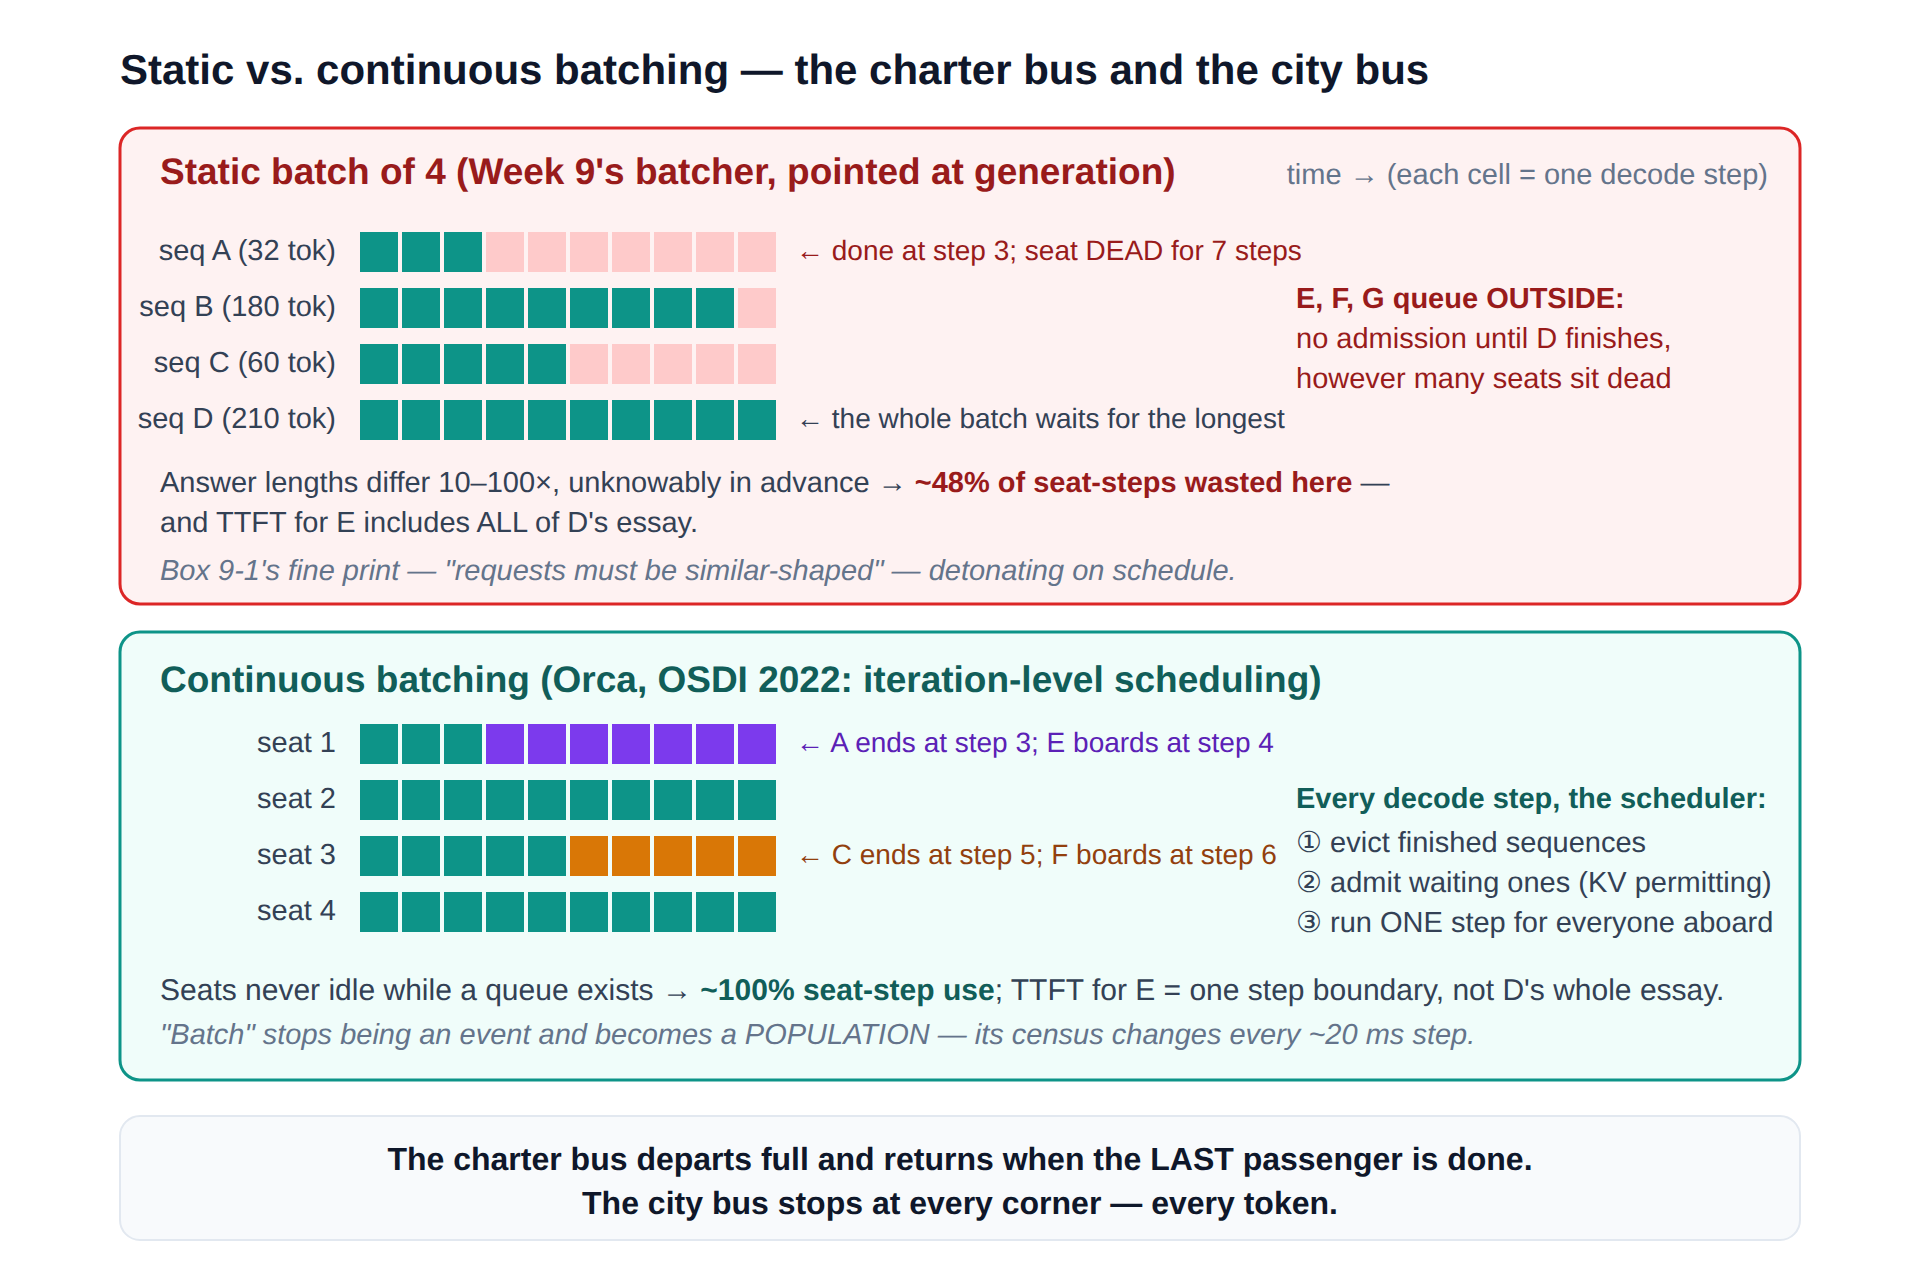
\includegraphics{figures/fig11-4_contbatch.png}}\\[3pt]
  \figcaption{그림 11-4  전세버스 대 시내버스. 정적 배치는 모두 함께 끝나거나 아무도 끝나지 않는다. 죽은 좌석과 대기 중 도착이 생기고 TTFT는 낯선 사람의 긴 글에 붙잡힌다. 반복 수준 스케줄링은 \textasciitilde{}20 ms 단계마다 승객 명단을 다시 정한다. 끝난 시퀀스가 내리고 기다리던 시퀀스가 타므로 대기열이 있는 동안 어느 좌석도 쉬지 않는다.}
\end{tbbfigure}

\subsection*{반복 수준 스케줄링 — Orca의 아름다운 아이디어 하나}

해결책은 Yu 등의 \textbf{Orca}(OSDI 2022)가 제시했다. 제9장의 더 읽을거리에서 "KV 캐시 강의 뒤"까지 미뤄 둔 논문인데, 그 강의가 20분 전에 끝났다. 해결책은 한 문장이다. \textbf{요청 스케줄링을 멈추고 반복을 스케줄링하라.} 디코드 루프는 이미 단계별로 실행되므로 \textit{어떤} 두 단계 사이에서도 배치 구성원을 바꿀 수 있다. 스케줄러는 \textasciitilde{}20 ms마다 세 박자의 주기를 실행한다. 방금 종료 토큰을 낸 시퀀스를 \textbf{퇴거}해 좌석과 KV 블록을 즉시 비운다. KV 풀이 수용할 수 있으면 기다리던 시퀀스를 \textbf{입장}시킨다. 이제 §11.3의 입장 규칙이 시스템을 지탱한다. 그리고 탑승한 모든 시퀀스를 순방향 패스 한 번으로 \textbf{진행}한다. 이것이 연속 배치다. "배치"는 시작과 끝이 있는 사건이 아니라 매 정류장에서 인구 조사가 달라지는 \textbf{집단}이 된다. 전세버스가 시내버스로 바뀌며 그림 11-4 위쪽의 두 실패 유형은 아예 일어날 수 없게 된다. 누군가 기다리는 동안 좌석이 쉬지 않고, 새 승객의 대기 시간은 낯선 사람의 글 길이가 아니라 \textit{단계} 단위로 측정된다.

왜 여기서는 \textit{가능}하지만 9주 차에는 불가능했는지 짚고 넘어갈 가치가 있다. CNN 순방향 패스는 \textbf{나눌 수 없는 커널 하나}의 실행이므로 Triton 동적 배처는 실행 도중에 퇴거하거나 입장시킬 수 없었다. 개입할 "단계 사이"가 없다. 반면 토큰마다 한 단계씩 도는 Python에서 보이는 바깥 루프라는 생성의 비효율은 스케줄링의 기회가 된다. 루프의 이음매가 스케줄러의 자리다. Orca의 두 번째 기여인 \textit{선택적 배치}는 길이가 다른 공존 시퀀스의 텐서 처리를 맡는다. 어텐션은 시퀀스별 캐시를 대상으로 시퀀스마다 실행하고, 큰 선형 계층은 모두를 함께 배치한다. vLLM 커널도 이 패턴을 이어받았다. 9주 차의 유산 하나는 변환 과정에서 사라진다. \textbf{max\_queue\_delay가 없어졌다.} 다음 출발까지 최대 한 단계뿐이므로 기다릴 이유가 없다. 후속 조절점은 \textit{한 단계에 얼마나 많은 작업을 태울 것인가}이며, 여기서 두 시계가 싸우기 시작한다.

\subsection*{프리필–디코드 간섭: 두 시계와 하나의 엔진}

새 스트림을 입장시키는 일은 공짜 좌석 배정이 아니다. 새 승객에는 50–350 ms의 연산 병목 GEMM인 \textbf{프리필}이 필요하다. 디코드 스트림 30개가 20 ms씩 나눠 쓰는 바로 그 GPU가 실행한다. 프리필을 나눌 수 없는 한 단계로 실행하면 모든 기존 스트림의 다음 토큰이 뒤에서 기다린다. 새 승객 한 명의 TTFT를 최소화하는 동안 30개 스트림이 \textbf{딸꾹질}하고 TPOT가 21에서 \textasciitilde{}250 ms로 치솟는다. 독자의 눈이 실제로 알아채는 끊김이다. 반대로 프리필을 미루면 디코드는 매끄럽지만 TTFT가 부푼다. 새로운 꼭짓점 이름으로 서빙 삼각형이 다시 태어난다. \textbf{TTFT 대 TPOT 대 비용}이다. 모서리를 따라 움직이는 조절점은 \textbf{청크 프리필(chunked prefill)}이다. 예를 들어 500토큰 프리필을 네 청크로 나누고 디코드 단계마다 한 청크를 함께 스케줄링한다. 새 승객의 프리필은 네 단계에 걸쳐 끝나 TTFT가 +\textasciitilde{}60 ms 늘지만 기존 승객의 TPOT는 단계마다 \textasciitilde{}2 ms만 증가한다. 엔진은 이 절충을 예산으로 노출한다. vLLM의 \code{max\_num\_batched\_tokens}는 \textit{반복마다 총 토큰 수(프리필 청크 + 디코드 단계)}를 제한한다. 이를 튜닝하는 일은 §9.3의 조절점 스윕이 다시 태어난 모습이며, 보고서의 지연 시간 시계가 하나가 아니라 둘이다.

\begin{terminalbox}
\begin{Verbatim}[breaklines=true,breakanywhere=true,fontsize=\small,formatcom=\color{tbbtermfg},codes=\tbbcodeactive]
# vLLM /metrics, sampled every 30 s while load ramps (c = 4 -> 64):
$ watch -n 30 'curl -s :8000/metrics | grep -E "running|waiting|cache"'

#            running   waiting   gpu_cache_usage    <- read as:
t+0:00          4          0          9 %           # roomy. TTFT=prefill
t+1:30         19          0         41 %           # filling. all admitted
t+3:00         31          0         88 %           # full-ish. TPOT sagging
t+4:30         32          9         97 %           # pool full: queue forms
t+6:00         32         26         98 %           # waiting grows: TTFT now
                                                    # queue-dominated (L=λW!)
# the three regimes every LLM service lives in: ROOMY (TTFT=prefill),
# FULL (TPOT shares bandwidth), QUEUED (TTFT explodes first).
# your SLO breaks in regime 3 at the TTFT clause - almost never TPOT.
\end{Verbatim}
\end{terminalbox}
\figcaption{터미널 기록 11-3  자체 메트릭으로 관찰한 연속 배치. running은 KV 풀의 좌석 수까지 올라간 뒤 멈추고, 풀이 차는 순간 waiting이 나타난다. 부하에서 실패하는 순서는 언제나 같다. 제7장의 하키 스틱 예측대로 대기열 때문에 TTFT가 먼저 무너진다.}

\subsection*{조절점은 무엇이 되었는가 — 9주 차 스윕의 변환}

\begin{tbbtablewrap}
  \begin{tabular}{@{}>{\raggedright\arraybackslash}m{\dimexpr 0.2447\tbltextwidth-2\tabcolsep\relax} >{\raggedright\arraybackslash}m{\dimexpr 0.2660\tbltextwidth-2\tabcolsep\relax} >{\raggedright\arraybackslash}m{\dimexpr 0.4894\tbltextwidth-2\tabcolsep\relax}@{}}
  \arrayrulecolor{tbbnavy}\specialrule{1pt}{0pt}{0pt}
  \rowcolor{tbbtablehead}{\centering \bfseries\color{tbbnavy}9주 차(동적 배치)} & {\centering \bfseries\color{tbbnavy}11주 차(연속 배치)} & {\centering \bfseries\color{tbbnavy}달라진 점과 이유} \\
  \arrayrulecolor{tbbnavy}\specialrule{0.7pt}{0pt}{2pt}
  {max\_batch\_size} & {\textbf{max\_num\_seqs}} & {좌석 수 — 다만 보통 KV 풀이 먼저 구속한다(§11.3). 주로 최악의 간섭을 제한한다} \\
  \arrayrulecolor{tbbtableborder}\hline
  {max\_queue\_delay} & {\textbf{(사라짐)}} & {기다릴 이유가 없다. 다음 출발까지 한 단계(\textasciitilde{}20 ms)뿐이다. 성공해서 사라진 조절점이다} \\
  \arrayrulecolor{tbbtableborder}\hline
  {(대응 항목 없음)} & {\textbf{max\_num\_batched\_tokens}} & {단계 예산: 반복마다 프리필 청크 + 디코드 토큰. TTFT ↔ TPOT 다이얼이다} \\
  \arrayrulecolor{tbbtableborder}\hline
  {memory.max (제5장, 외부)} & {\textbf{gpu\_memory\_utilization}} & {제한이 엔진 안으로 이동하며 반전되었다. 예산을 부여하면 엔진이 자체 좌석 수를 계산한다} \\
  \arrayrulecolor{tbbtableborder}\hline
  {(오버플로 시 충돌)} & {\textbf{선점 정책}} & {초과 인출 계획: 시퀀스 블록을 퇴거하고 나중에 다시 계산한다. 연산을 써서 메모리를 회수한다} \\
  \arrayrulecolor{tbbnavy}\specialrule{1pt}{2pt}{0pt}
  \end{tabular}\par
  \figcaption{표 11-1  변환된 배처 패널. 9주 차의 모든 직관은 11주 차에도 자리를 찾았지만 단위는 요청에서 토큰으로, 구속 자원은 연산에서 KV 풀로 이동했다.}
\end{tbbtablewrap}

§9.3의 배처에는 조절점이 두 개 있었고 연속 배처의 패널이 이를 변환한다. 좌석 수인 \textbf{max\_num\_seqs}가 max\_batch\_size를 잇는다. 하지만 §11.3에서 실제 상한은 대개 KV 풀임을 보았으므로 이 조절점은 주로 최악의 간섭을 제한한다. 단계 예산인 \textbf{max\_num\_batched\_tokens}는 TTFT↔TPOT 다이얼로서 max\_queue\_delay를 잇는다. \textbf{gpu\_memory\_utilization}은 풀 자체의 크기를 정한다. 제5장의 memory.max 규율이 이제 엔진 \textit{안쪽}으로 들어가 기분 좋게 반전되었다. 최악의 사용량을 측정해 제한을 정하는 대신 예산을 \textit{부여}하면 엔진이 자체 좌석 수를 계산한다. \textbf{선점 정책}은 풀의 초과 인출을 처리한다. vLLM은 시퀀스 전체의 블록을 퇴거하고 공간이 생기면 나중에 프리필을 \textbf{다시 계산}한다. 연산 비용을 내고 메모리를 회수하는 제3장 생각해 볼 문제의 답이 산업화되었다. 블록을 호스트 RAM으로 스왑하는 방법도 있지만 §10.2의 PCIe 계산을 보면 보통 재계산이 유리한 이유를 알 수 있다. 실습 스윕(§11.6)은 이 패널을 그대로 훑는다. 결과물은 9주 차 이후 모든 스윕과 같다. 의도적으로 찾은 굴곡점을 기록한다.

선점은 실제 모습으로 한 번 볼 가치가 있다. 개념을 배우기 전에 로그 줄로 먼저 만나게 되며, 이 문단을 읽지 않으면 오류로 오해할 수 있기 때문이다.

\begin{terminalbox}
\begin{Verbatim}[breaklines=true,breakanywhere=true,fontsize=\small,formatcom=\color{tbbtermfg},codes=\tbbcodeactive]
# push admission past the pool on purpose (c=48, long answers) and
# watch the engine's overdraft plan execute:
WARNING  Sequence group chatcmpl-8f21 is preempted by
         PreemptionMode.RECOMPUTE because there is not enough KV
         cache space. total_num_cumulative_preemption=1
INFO     Avg generation throughput: 691.2 tokens/s,
         Running: 31 reqs, Waiting: 17 reqs, GPU KV cache usage: 99.8%
# not a crash: one conversation's blocks were evicted; it will
# re-prefill when space frees. the victim's next tokens stall ~400 ms.
# occasional = healthy elasticity. CONSTANT = your pool is undersized:
# quantize the weights, shrink max-model-len, or buy the bigger card.
\end{Verbatim}
\end{terminalbox}
\figcaption{터미널 기록 11-4  실제 선점. WARNING은 설계가 작동한다는 뜻이다. 제3장의 OOM killer에는 더 부드러운 선택지가 없었지만 블록 관리자는 퇴거, 대기, 재프리필을 할 수 있다. 카운터를 활력 징후처럼 읽어라. 0에 가까우면 탄력적인 상태이고 계속 오르면 용량이 부족하다.}

정직하게 한계를 짚어 보자. 연속 배치는 \textit{길이가 제각각인 상황의 처리량}을 최적화한다. §11.3의 대역폭 계산을 폐기하지 않는다. 승객들이 메모리 버스 하나를 공유하므로 배치 1에서 32로 가면 TPOT는 여전히 \textasciitilde{}3× 나빠진다. \textbf{동승자가 없는} 워크로드에도 도움이 되지 않는다. 사용자 한 명의 에이전트 루프가 영원히 배치 1이라면 메모리 벽의 포로로 남는다. §11.5의 추측 디코딩이 바로 이 경우를 위해 존재한다. 엔진이 주는 선물은 더 좁지만 엄청나다. \textit{누군가 기다리는 동안 비용을 지불한 좌석이 절대 비지 않게} 보장한다. 좌석이 충분히 저렴한지는 여전히 제10장과 제12장의 몫이다.

\begin{calloutbox}{tbbpurple}{tbbpurplefill}
{\normalsize\bfseries\color{tbbpurple}생각해 보기}\par\vspace{3pt}
\begin{tbbitemize}
  \item 답변 길이가 32/180/60/210 tokens인 정적 배치(static batching) 4를 생각하라(그림 11-4). 정확한 좌석-단계 낭비와 10단계에 도착한 요청의 TTFT를 계산하고, 연속 배치에서 두 수치를 다시 계산하라. 이어 입력 길이별 버킷팅(제10장 규칙 ③)이 이 문제를 전혀 해결하지 못하는 이유를 설명하라.
  \item 2,000토큰 프롬프트에 chunk = 512 tokens인 청크 프리필을 적용한다. decode step ≈ 21 ms, prefill chunk ≈ 55 ms를 함께 스케줄링할 때 새 승객에게 추가되는 TTFT와 네 혼합 단계 동안 기존 승객의 TPOT를 추정하라. 이제 반대편을 주장하라. 언제 의도적으로 전체 프롬프트 프리필을 실행하겠는가? 힌트: 전용 프리필 레플리카는 상자 11-1의 DistServe 아이디어다.
  \item 터미널 기록 11-3의 구간 3은 running이 32에 고정되고 waiting=26인 상태다. W ≈ 4.4 s에서 L = λW를 사용해 도착률, 대기열 증가율, 26번째 대기자의 TTFT를 추정하라. 실패를 보고하는 SLO 조항은 무엇이며, 제12장은 어떤 해결책을 판매하는가?
  \item vLLM은 퇴거 후 재계산으로 선점한다. 3,000토큰 대화를 선점할 때 (a) 낭비되는 프리필 연산, (b) 피해자의 다음 턴 TTFT, (c) 공정성 측면에서 비용을 계산하라. 가장 최근, 가장 긴, 재계산 비용이 가장 싼 시퀀스 중 누구를 선점할지 정책을 설계하고 피해자에게 정당화하라.
\end{tbbitemize}
\end{calloutbox}

\section{PagedAttention과 vLLM: 운영체제가 안으로 들어가다}

지금까지 좌석이 귀중하다는 사실을 거듭 확인했다. §11.3은 KV 바이트로 가격을 매겼고 §11.4는 어느 좌석도 쉬지 않게 하겠다고 약속했다. 그러니 2023년 이전 엔진이 캐시를 \textit{저장}한 방식을 알면 아플 수밖에 없다. 입장할 때 시퀀스마다 \textbf{가능한 최대 길이에 맞춘 하나의 연속 슬랩}을 할당했다. 어텐션 커널이 깔끔한 스트라이드를 원해 연속 공간을 썼고, 입장 시 답변이 30 tokens일지 3,000일지 알 수 없어 최대 크기로 잡았다. 이미 본 영화다. malloc의 가장 오래된 비극이 예상대로 되풀이되었다. \textbf{내부 낭비}는 슬랩마다 예약했지만 쓰지 않는 꼬리다. 2,048을 예약해 180을 쓰면 91\%를 낭비한다. \textbf{외부 단편화}는 해제된 슬랩이 새 최대 크기 요청을 넣을 수 없는 틈을 남기는 현상이다. vLLM 저자들이 SOSP 2023 논문을 위해 프로덕션급 시스템을 측정했을 때 결과는 충격적이었다. \textbf{KV 메모리의 60–80\%가 유용한 것을 전혀 담지 않았다.} 애써 확보한 13 GB 풀이 4 GB처럼 동작했다. 버스 좌석의 절반 이상을 뜯어내 공기를 보관한 셈이다.

\begin{tbbfigure}
  \adjustbox{max width=0.94\linewidth,max totalheight=0.46\textheight}{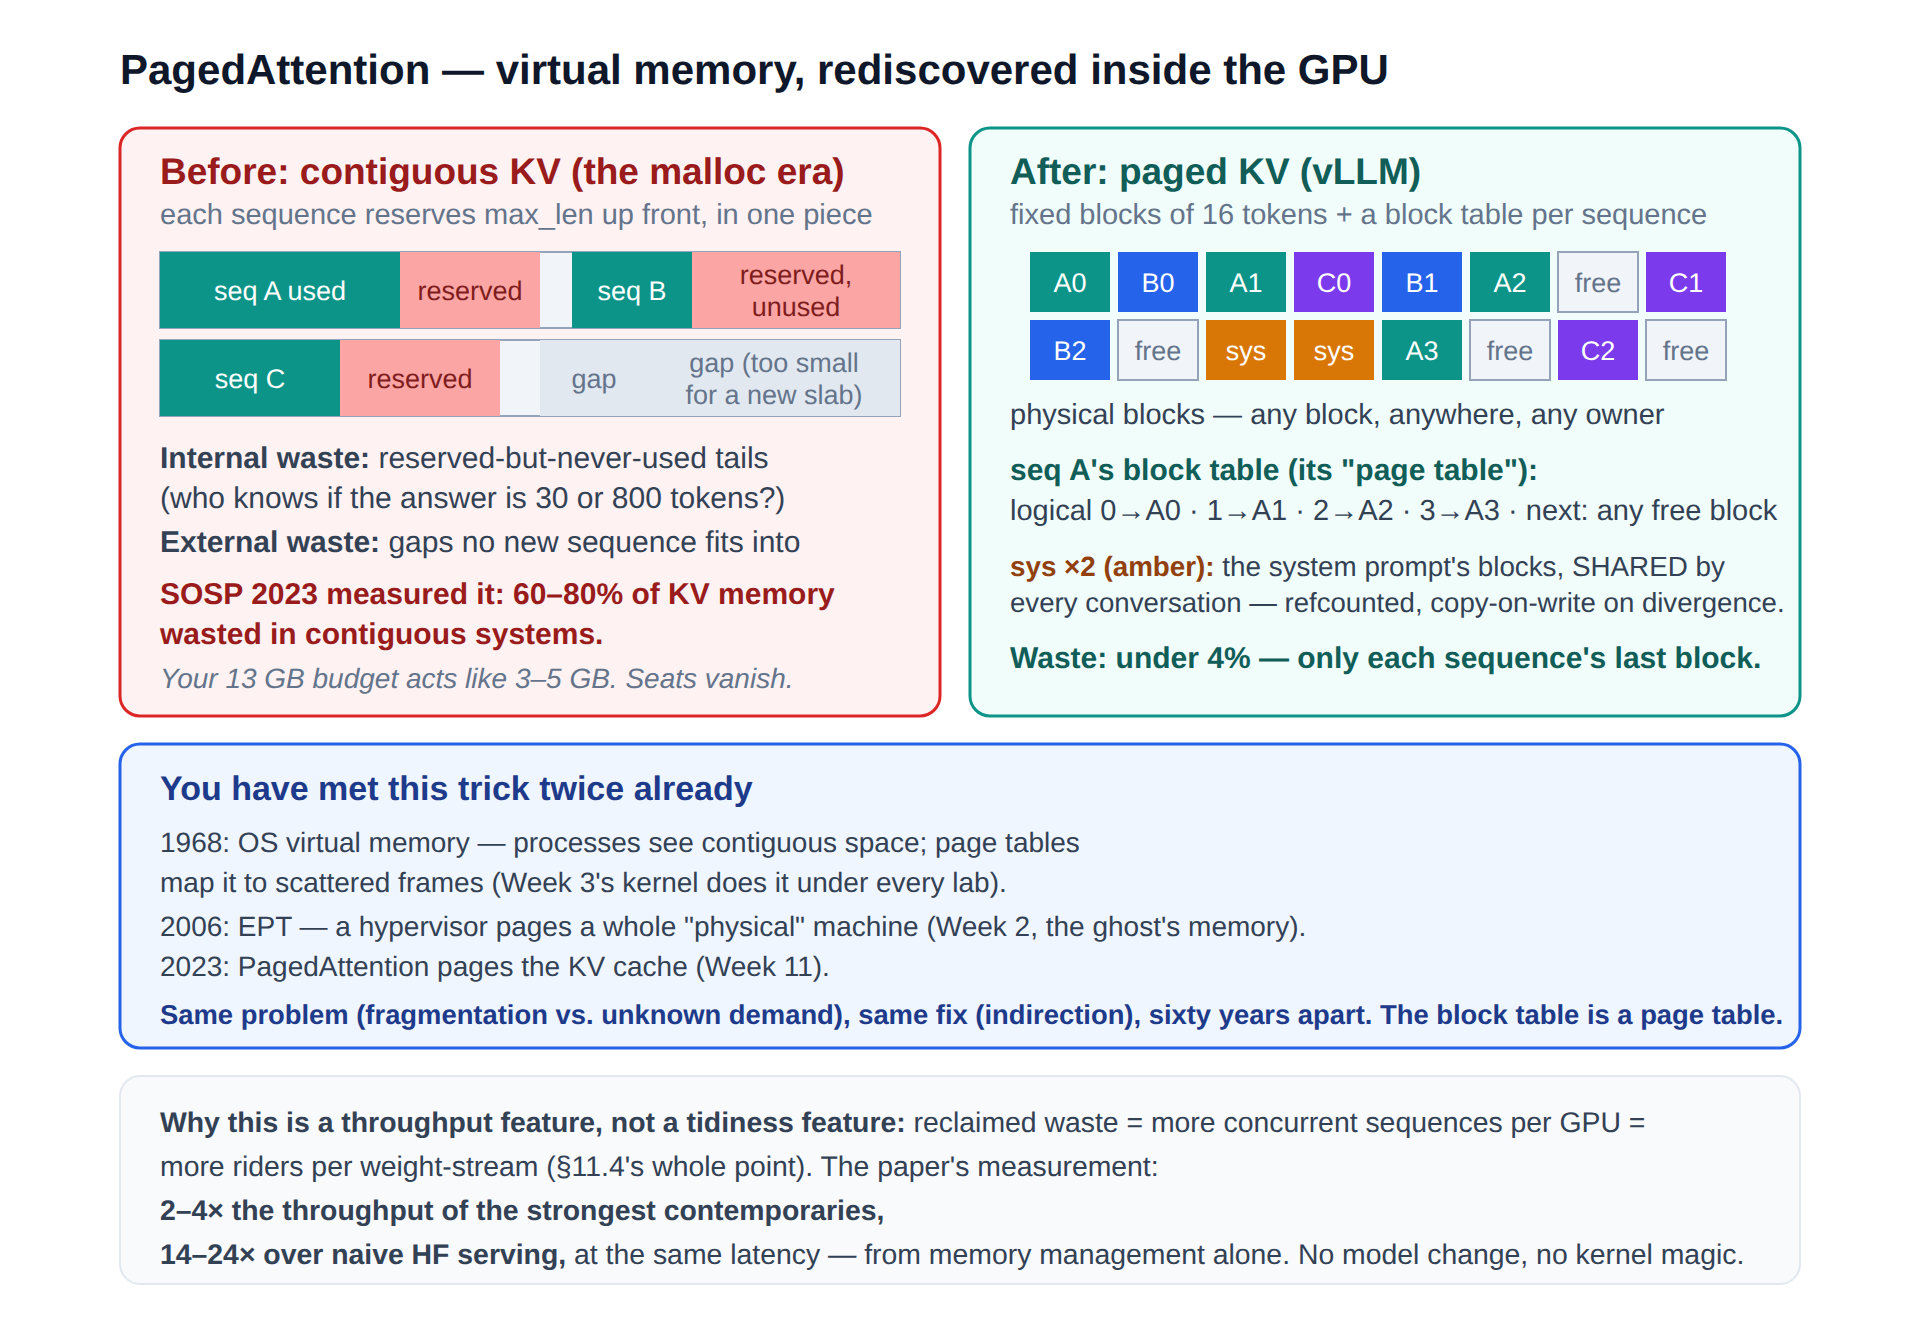
\includegraphics{figures/fig11-5_paged.png}}\\[3pt]
  \figcaption{그림 11-5  malloc 시대 대 페이징 시대. 연속 최대 길이 슬랩은 예약 꼬리와 쓸 수 없는 틈 때문에 풀의 60–80\%를 낭비한다. 고정 16토큰 블록과 시퀀스별 블록 테이블은 낭비를 4\% 아래로 줄이고, 복사 대신 참조 횟수로 공유할 수 있게 한다.}
\end{tbbfigure}

\subsection*{60년 된 해결책을 300 GB/s에 적용하다}

해결책은 컴퓨팅 역사상 가장 성공적인 간접 참조 기법이며, 이 책에서 이미 두 번 보았다. 운영체제는 1960년대부터 프로세스에 연속 물리 메모리를 주지 않았다. 고정 크기 \textbf{페이지}를 나눠 주고 \textbf{페이지 테이블}이 프로세스의 정돈된 가상 주소를 흩어진 물리 프레임에 대응시키게 했다. 그러면 단편화는 "마지막 페이지의 일부"로 줄어든다. 3주 차의 커널은 지금까지 실행한 모든 실습 아래에서 이를 수행한다. 2주 차에는 이 기법을 \textit{쌓아 올린} 모습도 보았다. EPT가 게스트 전체의 "물리" 메모리를 또 하나의 프로세스처럼 페이징했다. \textbf{PagedAttention}(Kwon et al., SOSP 2023)은 이를 통째로 어텐션에 이식한다. 제1장에서 필독으로 지정했고 이 책이 vLLM을 가르치는 이유가 된 논문이다. KV 풀을 \textbf{16 tokens}의 고정 블록으로 나누고, 각 시퀀스에 논리 위치 → 물리 블록을 대응시키는 \textbf{블록 테이블(block table)}을 주며, 어텐션 커널이 테이블을 따라가게 한다. 이제 시퀀스는 한 번에 \textit{블록} 하나씩 자라고 블록은 어디에나 놓일 수 있다. 낭비는 각 시퀀스의 덜 찬 마지막 블록으로 줄어 논문에서 \textbf{4\% 미만}으로 측정되었다. 모델도 정밀도도 바꾸지 않고 장부 관리만 바꿨다. 좌석의 효과가 누적되므로 처리량 개선은 제10장만큼 크다. 낭비를 회수하면 같은 풀에 2–3× 더 많은 동시 시퀀스가 들어가고, 그만큼 많은 승객이 매 20 ms 가중치 스트림을 상각한다. 종단 간 측정에서 \textbf{같은 지연 시간으로 당시 가장 강력한 시스템보다 2–4×, 단순 HF 서빙보다 14–24× 높은 처리량}을 냈다. 해당 세대 최고의 서빙 시스템 논문은 본질적으로 메모리 할당기에 관한 논문이다. cgroup을 다룬 제3장부터 이 책이 강조해 온 감각과 정확히 같다.

\subsection*{공유: 블록 테이블의 두 번째 묘기 — 제6장의 빚을 갚다}

페이지 테이블은 단편화를 없애는 것보다 더 많은 일을 운영체제에 해 주었다. 두 프로세스가 같은 물리 프레임을 매핑한 덕분에 Unix 공유 라이브러리와 쓰기 시 복사 fork가 가능해졌다. 블록 테이블도 이를 재현한다. 제품의 모든 대화가 같은 \textbf{900-token 시스템 프롬프트}로 시작한다고 하자. 연속 슬랩은 이를 32번 저장한다. 32 × 900 × 112 KB ≈ \textbf{동일한 바이트 3.2 GB}로 4k 좌석 거의 일곱 개가 순수 중복에 쓰인다. 페이징하면 900토큰은 \textbf{참조 횟수}가 붙은 \textasciitilde{}57개 블록이 된다. 모든 대화의 테이블이 \textit{같은} 물리 블록을 가리키므로 \textbf{한 번만} 저장한다(≈ 101 MB). 갈라지는 시퀀스에는 블록 단위 \textbf{쓰기 시 복사}를 적용한다. 이것이 \textbf{접두사 캐싱}이며 두 번 보상한다. 먼저 메모리 좌석 6개 이상을 회수한다. 그리고 \textit{시계}도 줄인다. 접두사가 이미 상주한 새 대화는 \textbf{그 접두사의 프리필을 완전히 건너뛰어} TTFT에서 연산 \textasciitilde{}100 ms를 없앤다. 돌아온 대화의 5번째 턴은 3,000토큰 기록 전체가 아니라 새 접미사만 다시 프리필한다. §11.3의 다중 턴 세금을 대부분 돌려받는다.

이로써 제6장에서 보류해 둔 고정 세션의 긴장을 해결할 수 있다. 캐시된 블록은 \textbf{한 레플리카의 VRAM}에 산다. 그렇다면 라우터가 대화를 레플리카에 고정해야 할까? 업계가 수렴한 성숙한 답은 \textbf{정확성은 상태 비저장으로 유지하고 어피니티는 성능 힌트로만 쓴다}는 것이다. 요청은 여전히 전체 기록을 담으므로 \textit{어떤} 레플리카도 5번째 턴을 정확히 처리할 수 있다. 캐시 미스는 접미사 하나가 아니라 \textit{전체} 프리필(\textasciitilde{}350 ms)의 비용을 내게 하지만 잘못된 답을 만들지는 않는다. 따라서 대화 id에 일관된 해시를 적용하는 세션 해시 라우팅은 편할 때 순수한 이점이고, 그렇지 않아도 해 없이 성능만 저하된다. 롤아웃, 스케일 다운, 레플리카 사망이라는 제6장 고정 상태의 세 재앙도 접두사 적중률을 잠시 낮출 뿐이다. 제6장에서 경고한 설계, 즉 잃으면 대화가 깨지는 세션 \textit{저장소}와 비교해 보자. "고정"이라는 말은 같지만 엔지니어링은 반대다. \textbf{캐시를 계약으로 만들지 마라.}

\subsection*{기관별로 살펴보는 vLLM — 추측이라는 수단}

이 장의 내용을 조립하면 vLLM의 블록 다이어그램(그림 11-6)이 나온다. 제9장의 여섯 기관 중 두 기관을 이식한 구조다. \textbf{배처}는 §11.4의 반복 스케줄러다. \textbf{모델 저장소}의 핫 경로에는 §11.5의 테이블, 참조 횟수, 선점을 실행하는 VRAM 속 "운영체제"인 블록 관리자가 생겼다. 주변은 익숙하다. OpenAI 호환 프런트 도어가 SSE로 통신하므로 제6장의 클라이언트, LB, 타임아웃 교훈이 그대로 적용된다. 제6장의 safetensors 로딩과 터미널 기록 11-3에서 이미 이름을 읽은 Prometheus 메트릭도 있다. 실행기 안에서는 제10장의 두 기법이 제값을 한다. 디코드 단계는 \textbf{CUDA Graphs}로 캡처한다. 3B 디코드 단계는 21 ms 예산 안에서 수백 개의 작은 커널을 실행하므로 실행 오버헤드가 중요한 적이다. 그래프가 전체 단계를 제출 한 번으로 재생해 제10장의 \textit{a}를 빌드가 아니라 런타임에서 줄인다. 가중치 슬롯은 제10장에서 그룹별 스케일 용어를 배운 \textbf{GPTQ/AWQ INT4} 산출물을 받는다. 책의 모델은 INT4에서 \textasciitilde{}1.9 GB이므로 배치 1 단계 트래픽이 \textasciitilde{}2.4 GB → \textbf{\textasciitilde{}8 ms → tokens/s 2.5×}로 줄고, KV 풀은 4 GB 넓어져 4k 좌석이 ≈ 9개 늘어난다. 게이트를 거친 산출물 하나가 두 시계와 좌석 수를 모두 개선한다. 퍼플렉시티나 작업 지표를 명시한 허용 오차와 비교하는 §10.3의 게이트는 그대로 적용된다.

실행기의 한 줄은 별도 문단을 쓸 가치가 있다. 제10장의 마지막 약속을 갚고 §11.2의 "본질적으로 직렬"이라는 규칙을 조금 휘게 하는 \textbf{추측 디코딩}이다. 핵심은 메모리 벽의 비대칭에서 차익을 얻는 것이다. 디코드 단계의 20 ms는 토큰 하나의 \textit{대역폭}을 사지만 수백 토큰 분량의 \textit{FLOP}도 함께 산다. AI ≈ 1이고 능선이 400이므로 연산 비용은 이미 냈지만 유휴 상태다. 아주 작은 \textbf{초안 모델(draft model)}(예: \textasciitilde{}160M, \textasciitilde{}1 ms/token)이 k = 4 tokens를 저렴하게 추측하게 한 뒤, 목표 모델이 \textbf{네 개를 한 패스에서 모두 검증}하게 한다. 토큰 \textit{하나}를 생성할 때와 같은 6 GB를 스트리밍한다. 가장 긴 올바른 접두사를 받아들이고 표본 추출을 보정해 출력 분포가 \textit{증명 가능하게 동일}하도록 만든다. 품질 절충이 아니라 시스템 기법이다. 일반 텍스트에서는 네 개 중 \textasciitilde{}3개가 살아남는다. 유효 비용은 (4 × 1 ms 초안) + (21.5 ms 검증 한 번) ≈ \textasciitilde{}3 tokens당 25.5 ms이므로 \textbf{\textasciitilde{}8.5 ms/token, 배치 1에서 TPOT 2.5× 개선}이다. 전부 낭비될 뻔한 FLOP으로 샀다. 정직한 작은 글씨도 있다. 어렵거나 특이한 텍스트에서는 수락률이 무너져 초안 비용은 내면서 속도 향상 → 1×가 된다. 초안 모델도 VRAM을 차지하며, 배치가 높을수록 유휴 FLOP 보조금이 줄어든다. 그래서 추측은 \textit{단일 사용자 에이전트 루프}의 수단이고, 다수 사용자를 위한 연속 배치와 대체로 상호 보완적이다.

\begin{calloutbox}{tbbpurple}{tbbxF5F3FF}
{\normalsize\bfseries\color{tbbx5B21B6}상자 11-1  더 넓은 LLM 서빙 선택지 — 이 책에서 선반에 남겨 둔 수단}\par\vspace{3pt}
남은 주에는 제12장이 필요하므로 여기서는 각 기법을 한 줄로 정직하게 설명한다. 나중에 만났을 때 아이디어와 대가를 알아볼 정도면 충분하다.

\begin{tbbitemize}
  \item \textbf{분리형 프리필(DistServe 방식):} 프리필과 디코드를 \textit{별도의 레플리카 풀}에서 실행한다. §11.2의 두 장치를 물리적으로 분리해 서로 간섭하지 않게 한다. 그 대가로 프리필한 KV 캐시를 네트워크 너머로 전달해야 한다. §10.2의 PCIe 교훈을 클러스터에 적용한 셈이다.
  \item \textbf{Multi-LoRA 서빙:} 하나의 기본 모델 가중치와 KV 풀을 수십 개의 미세 조정 어댑터가 공유하는 S-LoRA 기법이다. 어댑터는 수 메가바이트이므로 "고객마다 모델 하나"가 더 이상 "고객마다 GPU 하나"를 뜻하지 않는다.
  \item \textbf{구조화/유도 디코딩:} 문법이나 JSON 스키마로 표본 추출을 제한한다. 단계별 토큰 마스크에 작은 비용을 내고 에이전트 파이프라인의 출력 유효성을 얻는다. SGLang의 RadixAttention은 프로그램 형태 호출 사이에서 적극적인 접두사 재사용과 이를 결합한다.
  \item \textbf{KV 오프로딩과 계층화:} 차가운 대화의 블록을 호스트 RAM이나 NVMe로 내보내고 다음 턴에 복원한다. §10.2의 PCIe 바이트와 §11.3의 재프리필 연산을 절충한다. 블록 테이블 덕분에 말 그대로 페이징 정책이 된다.
\end{tbbitemize}

모든 기법은 이 장의 세 기본 요소인 두 단계 루프, 블록 테이블, 반복 스케줄러를 다시 조합한 것이다. 기본 요소를 익혀라. 제품은 낡아도 기본 요소는 낡지 않는다.
\end{calloutbox}

\vspace{3.0pt}

\begin{tbbfigure}
  \adjustbox{max width=0.94\linewidth,max totalheight=0.46\textheight}{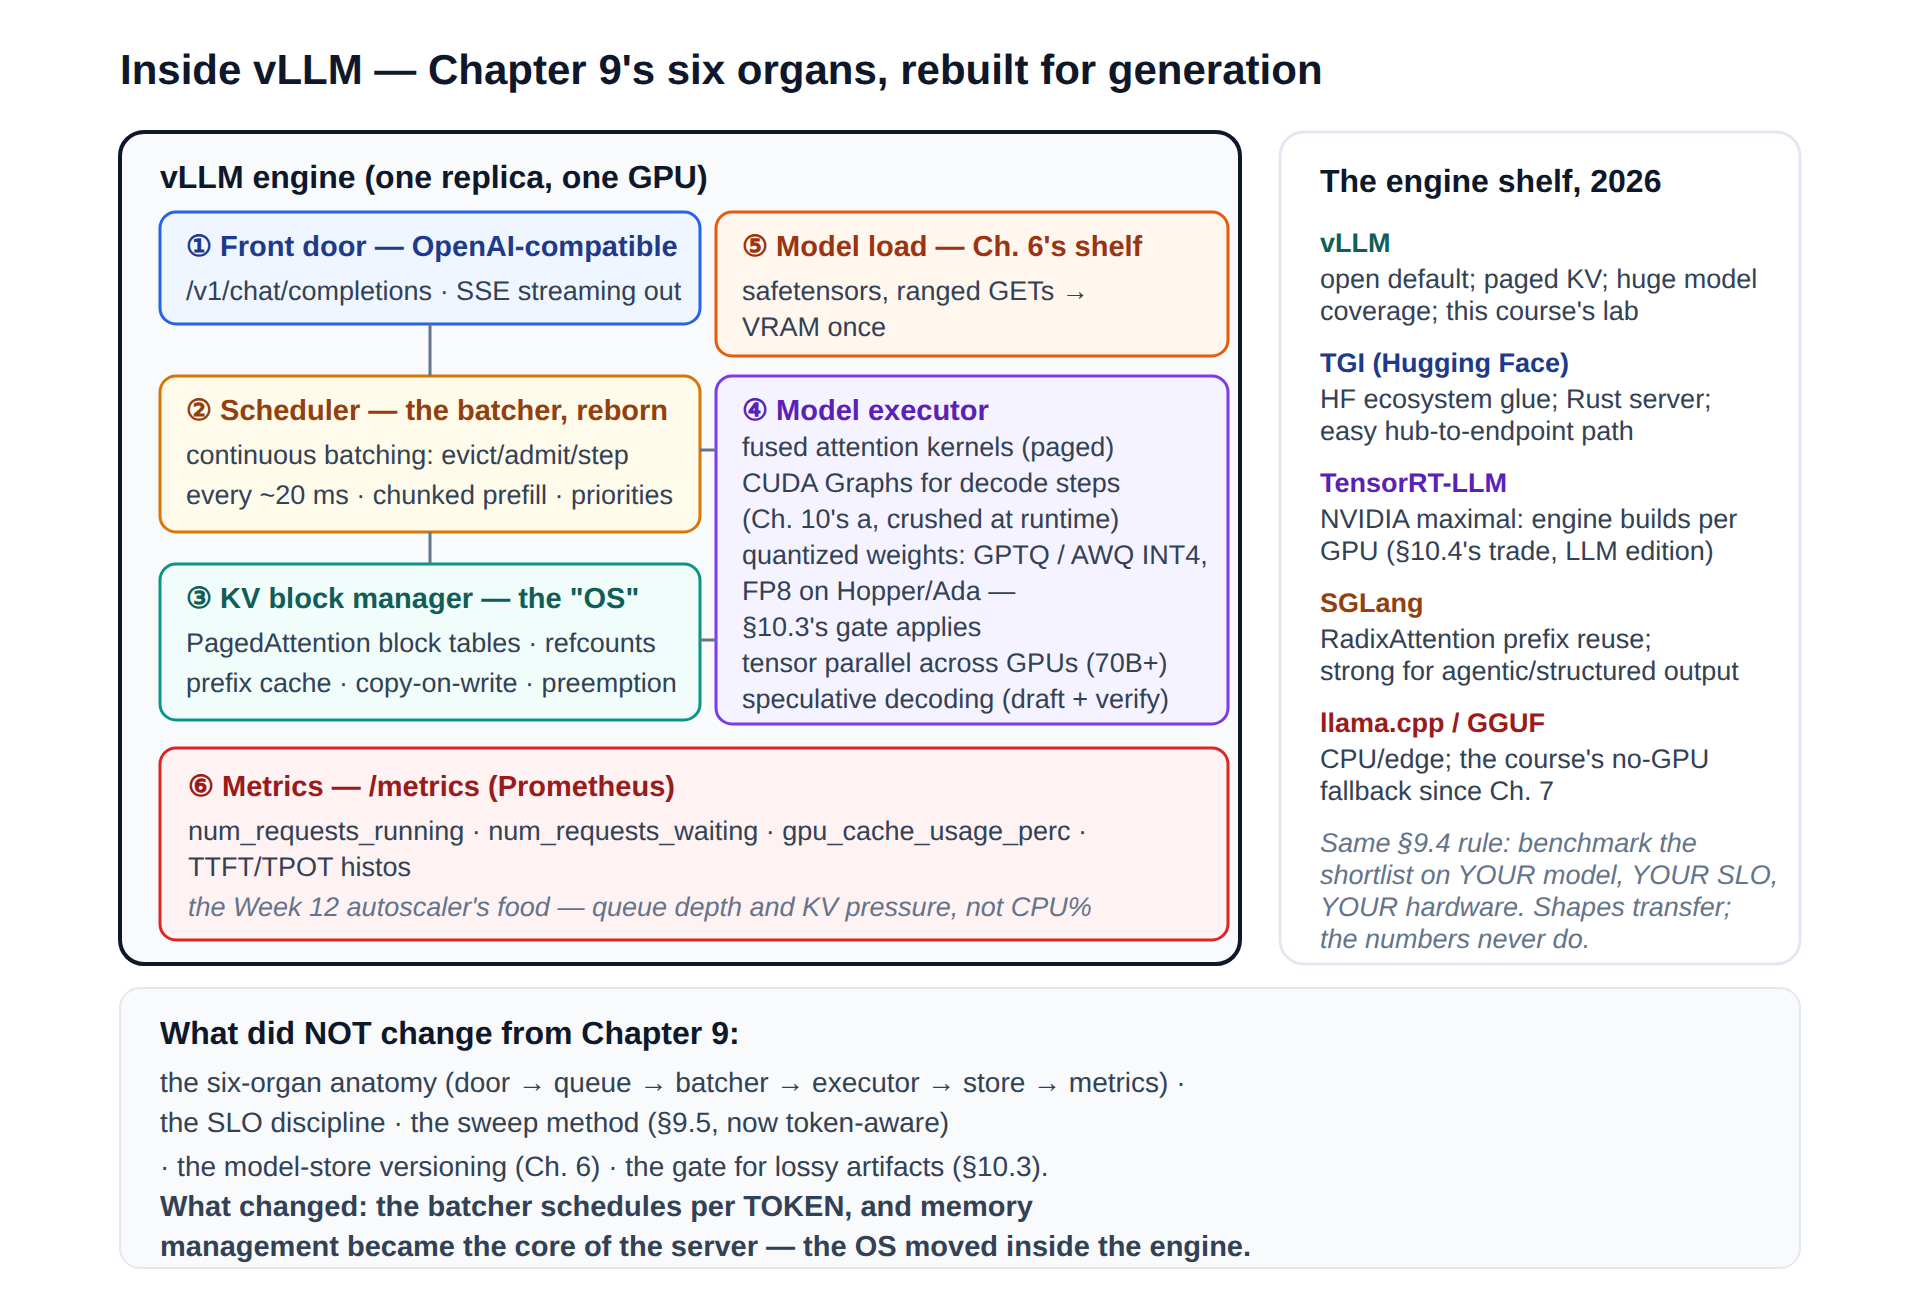
\includegraphics{figures/fig11-6_vllm.png}}\\[3pt]
  \figcaption{그림 11-6  제9장의 구조를 다시 만든 vLLM. 배처는 토큰마다 스케줄링하고 블록 관리자는 페이지 테이블을 실행하며 메트릭은 12주 차 오토스케일러에 공급된다. 오른쪽은 2026년의 엔진 선택지다. §9.4의 같은 규칙에 따라 자신의 모델, SLO, 하드웨어에서 후보를 벤치마크해야 한다.}
\end{tbbfigure}

vLLM 주변의 선택지(그림 11-6 오른쪽)를 제9장의 방식으로 간단히 살펴보자. \textbf{TGI}는 Hugging Face의 접착제로, 그 생태계에서 허브부터 엔드포인트까지 가장 짧은 경로다. \textbf{TensorRT-LLM}은 §10.4의 절충을 LLM 규모에 적용한다. GPU마다 엔진을 빌드해 최대 성능의 커널을 얻고 좁은 범위도 함께 받아들인다. Hopper/Ada 실리콘에서 \textbf{FP8}이 제값을 하는 곳이다. 가중치와 KV 캐시에 모두 적용한다. 표 10-1의 "11주 차 FP8은 여기서 동작한다"는 예고가 실현되었다. 플릿의 L4에도 회로가 있으며 같은 §10.3 게이트가 적용된다. \textbf{SGLang}은 호출이 프로그램처럼 보일 때 앞선다. 에이전트, 많이 공유하는 접두사, 스키마에 묶인 출력이 해당한다. \textbf{llama.cpp/GGUF}는 제7장 이후 GPU가 없을 때 쓰는 대안으로 남아 있다. 선택 규칙은 §9.4 이후 변하지 않았고 앞으로도 변하지 않는다. \textit{자신의 모델, SLO, 하드웨어에서 후보를 벤치마크하라. 형태는 옮겨 가지만 수치는 그렇지 않다.} 이 책이 vLLM으로 실습하는 이유는 개방형 기본값이고, 메트릭이 개념을 가르치며, 논문 자체가 이 장의 내용이기 때문이다.

\begin{calloutbox}{tbbpurple}{tbbpurplefill}
{\normalsize\bfseries\color{tbbpurple}생각해 보기}\par\vspace{3pt}
\begin{tbbitemize}
  \item max\_len 2,048 슬랩을 사용하는 연속 엔진이 [30, 2,000] tokens에서 균일한 길이의 답변을 서빙한다. 시퀀스당 기대 내부 낭비와 L4의 13 GB 풀에서 잃는 좌석 수를 16토큰 페이징 블록과 비교하라. 이어 블록 크기가 1이나 512가 아니라 16인 이유와 각 극단의 비용을 설명하라.
  \item 제품 A/B 테스트에서 접두사 캐싱은 평균 TTFT를 38\% 줄였지만 p99 TTFT는 6\%만 줄였다. §11.4의 구간과 레플리카별 적중률 분포로 두 수치를 설명하라. LB 설정 한 줄로 p99를 가장 크게 개선할 라우팅 변경도 제시하라.
  \item 추측 디코딩은 "출력 분포를 보존함이 증명"되었지만 §10.3은 모든 손실 변경에 게이트를 요구했다. 추측은 손실 변환인가? 배포 전에 여전히 검증해야 할 사항을 제시하라. 지연 시간 분포, 토큰당 비용, 수락률 텔레메트리를 고려하고 조용한 실패 유형을 감지할 대시보드 항목도 말하라.
  \item L4 한 대의 Multi-LoRA 입장 정책을 설계하라. 기본 모델은 6 GB, 어댑터는 각각 40 MB이며 KV 풀을 공유한다. 고객 어댑터에는 캐시할 수 있는 300토큰 시스템 접두사가 있다. 어댑터 수가 늘수록 좌석은 어디로 가는가? "기본 모델 하나와 여러 어댑터"가 "기본 모델을 양자화해 좌석을 더 확보"하는 방식보다 유리해지는 지점도 계산으로 개략적으로 나타내라.
\end{tbbitemize}
\end{calloutbox}

\section{실습: 실제 LLM 서빙, 스트리밍, 측정}

이번 실습은 9주 차와 10주 차와 결이 다르다. vLLM은 \code{pip install} 한 번이면 되므로 빌드할 것이 없다. 따라서 \textbf{모든 시간을 측정에 쓴다.} 결과물은 수치로 뒷받침한 프로젝트의 새 SLO 문장이다. 수업용 T4에서 작은 오픈 모델을 서빙한다. Qwen2.5-1.5B-Instruct는 게이트가 없고 FP16에서 3.1 GB라 16 GB 안에서 KV 풀과 함께 여유롭게 들어간다. 직접 눈으로 스트리밍한 뒤 9주 차에 시계 하나를 측정했던 것처럼 두 시계를 측정한다. GPU 시간 예산은 \textasciitilde{}\$2–3이며 언제나처럼 결제 내역 스크린샷을 제출한다.

\begin{tbbfigure}
  \adjustbox{max width=0.94\linewidth,max totalheight=0.46\textheight}{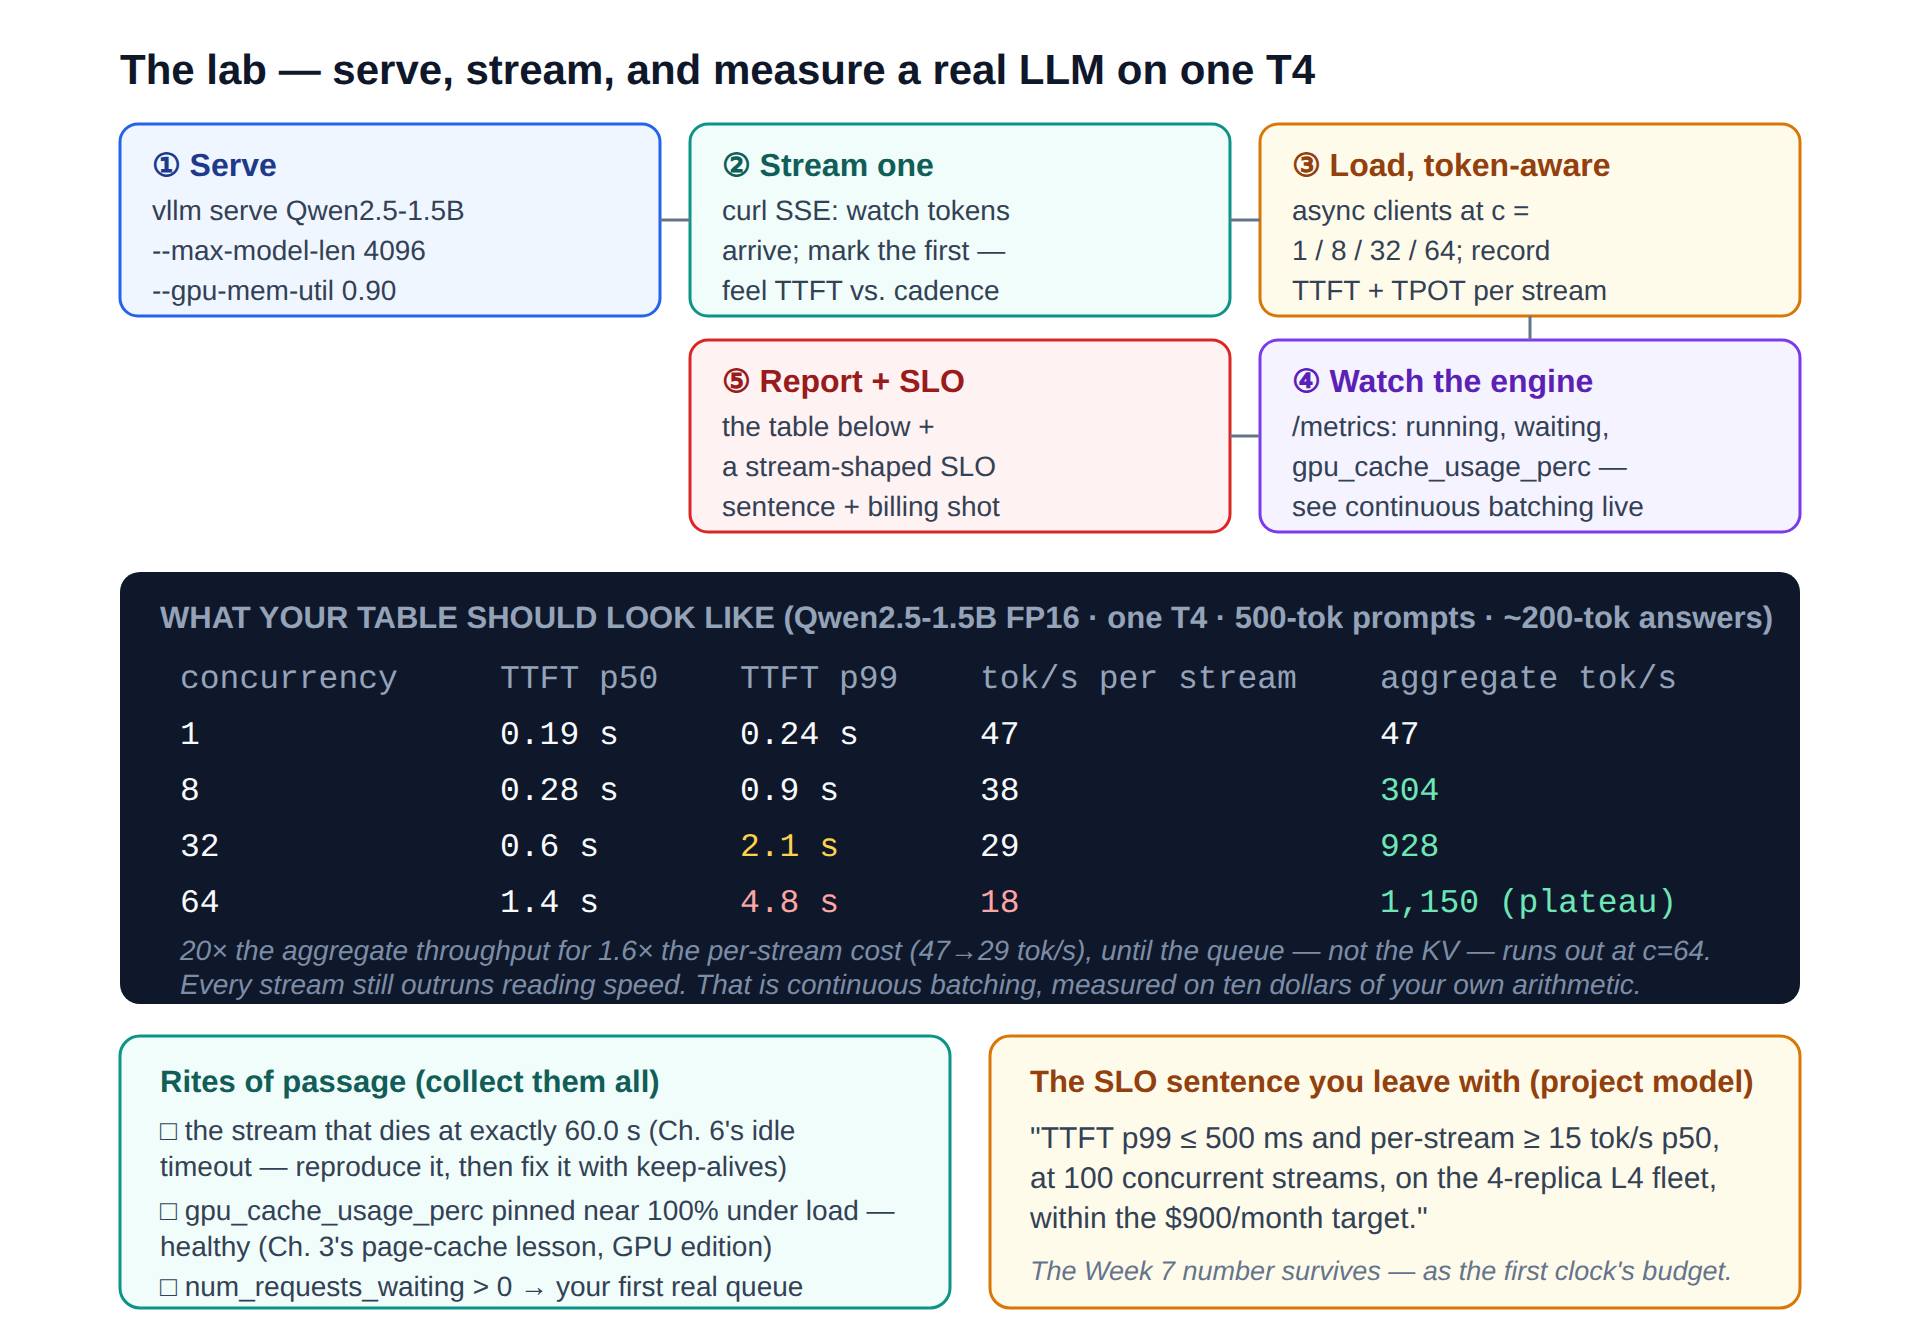
\includegraphics{figures/fig11-7_lab.png}}\\[3pt]
  \figcaption{그림 11-7  실습 파이프라인과 예상되는 결과의 형태. 서빙하고, 하나를 손으로 스트리밍하고, 토큰 인식 부하 테스트를 실행하며, 엔진의 자체 집계를 관찰한다. 마지막에는 표, SLO 문장, 두 가지 통과 의례를 남긴다.}
\end{tbbfigure}

\subsection*{일곱 단계}

\begin{tbbitemize}
  \item \textbf{① 서빙한다.} \code{vllm serve Qwen/\allowbreak Qwen2.5-1.5B-Instruct --max-model-len 4096 --gpu-memory-utilization 0.90}을 실행한다. 시스템 엔지니어처럼 부팅 로그를 읽는다. 가중치 로드(제6장의 범위 GET), CUDA 그래프 캡처(제10장의 a), \textbf{풀이 보유한 KV 블록 수}를 출력하는 줄을 확인한다. 터미널 기록 11-2의 계산을 엔진이 대신 해 준 결과다. 시작에는 1분 이상 걸리므로 제5장의 준비 상태 프로브 예산을 떠올려야 한다.
  \item \textbf{② 하나를 손으로 스트리밍한다.} 터미널 기록 11-5처럼 \code{"stream": true}와 \code{curl -N}을 사용하고 SSE 청크가 도착하는 모습을 \textit{지켜본다}. 잠깐 숨을 고른 뒤 첫 청크(TTFT)가 오고 이어 일정한 가랑비(TPOT)가 내린다. 어떤 하네스(harness)가 추상화하기 전에 두 시계를 직접 눈으로 본다.
  \item \textbf{③ 직접 캐시 크기를 계산한다.} 모델 카드에 맞춰 kv\_math.py를 실행한다. 28개 계층에 KV 헤드 2개 × 128이므로 작은 모델의 캐시는 \textasciitilde{}28 KB/token으로 3B의 4분의 1이다. ①단계에서 엔진이 출력한 블록 수를 예측하고 10\% 안에서 맞춘다. 틀리더라도 실습에서 가장 저렴한 교훈이다. 빠뜨린 항을 찾으면 되며 보통 활성값이다.
  \item \textbf{④ 토큰을 인식하는 방식으로 부하를 건다.} 제공된 비동기 하네스는 c = 1 / 8 / 32 / 64개의 동시 스트림을 연다. 500토큰 프롬프트와 \textasciitilde{}200토큰 답변을 사용하고 길이를 통제하기 위해 \code{ignore\_eos}를 적용한다. 이 사실을 보고서에 명시해야 한다. 요청 지연 시간이 아니라 \textbf{스트림별 TTFT와 TPOT 백분위수}를 기록한다. Locust의 요청 수준 관점은 구조적으로 이 상황을 볼 수 없다. 하네스는 aiohttp 50줄이고, 이를 읽는 것도 실습에 포함된다.
  \item \textbf{⑤ ④가 실행되는 동안 집계를 지켜본다.} 터미널 기록 11-3의 세 구간을 실시간으로 재현한다. \code{running}은 좌석 수까지 올라가고, 풀이 차면 \code{waiting}이 나타나며, \code{gpu\_cache\_usage\_perc}는 높은 값에 고정된다. \textbf{높은 값에 고정되는 것은 정상}이다. 제3장의 페이지 캐시 교훈을 GPU에 적용한 모습이다. TTFT p99가 느끼는 것은 캐시가 아니라 대기열이다.
  \item \textbf{⑥ 통과 의례를 수집한다.} 앞에 60초 유휴 LB나 프록시를 두거나 실습 자료의 nginx 설정을 사용해 \textbf{정확히 60.0 s에 끊기는 스트림}을 재현한다. SSE keep-alive 주석을 추가하고 유휴 타임아웃을 높여 고친다. 제6장의 빚을 직접 갚는 과정이다. 선택 사항이지만 같은 모델의 \textbf{AWQ INT4} 빌드로 스윕 한 행을 반복하고 두 TPOT를 나란히 비교하기를 권장한다. 보고서에서는 이 비교 옆에 §10.3의 게이트 논의를 넣어야 한다.
  \item \textbf{⑦ 보고서와 문장을 작성한다.} 그림 11-7의 표에는 각 c에서 TTFT p50/p99, 스트림별 tok/s, 집계 tok/s를 넣는다. 이어 형태의 원인을 밝히는 문단 하나를 쓴다. c가 증가할수록 스트림별 TPOT는 어디로 갔는가? TTFT의 굴곡점은 어디에 나타났으며 왜 대기열 때문인가? 각 조항을 뒷받침하는 측정 근거와 함께 프로젝트의 SLO 문장을 다시 쓴다. 추정 → 측정 → 최적화 → \textbf{재계약}으로 이어지며, 제안서의 비용 이야기가 이제 스트림 단위로 말한다.
\end{tbbitemize}

\begin{terminalbox}
\begin{Verbatim}[breaklines=true,breakanywhere=true,fontsize=\small,formatcom=\color{tbbtermfg},codes=\tbbcodeactive]
$ vllm serve Qwen/Qwen2.5-1.5B-Instruct --max-model-len 4096 \
      --gpu-memory-utilization 0.90
INFO  Loading weights: 3.09 GiB in 14.2 s (Ch. 6's shelf at work)
INFO  # GPU blocks: 21,856  (= 349,696 tokens of KV pool)   # step ③!
INFO  Capturing CUDA graphs for decode... done (Ch. 10's a, crushed)
INFO  Uvicorn running on http://0.0.0.0:8000

$ curl -N localhost:8000/v1/chat/completions -H "Content-Type: application/json" \
   -d '{"model":"Qwen/Qwen2.5-1.5B-Instruct","stream":true,
        "messages":[{"role":"user","content":"What is a KV cache?"}]}'
data: {"choices":[{"delta":{"content":"The"}}]}          <- ~0.18 s: TTFT
data: {"choices":[{"delta":{"content":" KV"}}]}          <- then a steady
data: {"choices":[{"delta":{"content":" cache"}}]}       <-   ~21 ms drizzle
  ...
data: [DONE]
# you have now SEEN both clocks. everything else is percentiles.
\end{Verbatim}
\end{terminalbox}
\figcaption{터미널 기록 11-5  손으로 서빙하고 스트리밍하기. 부팅 로그는 KV 블록 수를 알려 주므로 직접 계산한 결과와 맞춰야 한다. SSE 스트림은 TTFT와 TPOT를 물리적으로 느끼게 한다. 한 번 숨을 고른 뒤 읽기보다 빠른 가랑비가 이어진다.}

\begin{terminalbox}
\begin{Verbatim}[breaklines=true,breakanywhere=true,fontsize=\small,formatcom=\color{tbbtermfg},codes=\tbbcodeactive]
$ python sweep.py --url :8000 --conc 1 8 32 64 --prompt-tok 500 --gen-tok 200
 c    TTFT p50   TTFT p99   TPOT p50    per-stream   aggregate
  1     0.19 s     0.24 s    21.4 ms      47 tok/s      47 tok/s
  8     0.28 s     0.90 s    26.3 ms      38 tok/s     304 tok/s
 32     0.60 s     2.10 s    34.5 ms      29 tok/s     928 tok/s
 64     1.40 s     4.80 s    55.6 ms      18 tok/s   1,150 tok/s  (plateau)
# read it with the chapter: aggregate x20 for per-stream /1.6 (c=32);
# TTFT p99 dies FIRST (queueing - regime 3), TPOT never falls below
# reading speed; and the plateau is §11.3's bandwidth, not "load".
# now write the SLO sentence your own numbers can sign.
\end{Verbatim}
\end{terminalbox}
\figcaption{터미널 기록 11-6  토큰 인식 스윕. 9주 차 방법을 두 시계 너비로 확장했다. 굴곡점은 TTFT p99의 대기열에, 고원은 집계 tokens/s의 메모리 버스에 있다. SLO 문장은 홍보 자료가 아니라 표에서 나온다.}

\begin{calloutbox}{tbbred}{tbbxFEF2F2}
{\normalsize\bfseries\color{tbbx991B1B}상자 11-2  보고서의 위험 신호 — 스트리밍판 채점자 점검표}\par\vspace{3pt}
\begin{tbbitemize}
  \item \textbf{스트리밍 엔드포인트 주변에 요청 수준 p99 사용} — 자신의 보고서에서 사례 11-A의 실수를 반복한 것이다.
  \item \textbf{TTFT와 TPOT를 함께 평균 냄} 또는 수식어 없이 "지연 시간"이라 표현 — 두 시계와 두 분포가 있으며 하나의 수치로 합치지 않는다.
  \item \textbf{단일 스트림 tokens/s를 용량으로 제시} — 용량은 동시 부하에서 집계한 값이며 스트림별 하한도 명시해야 한다.
  \item \textbf{통제하지 않은 답변 길이를 밝히지 않고 스윕} — ignore\_eos나 길이 분포를 명시하라. 숨겨진 변동 위의 백분위수는 정장을 입은 잡음이다.
  \item \textbf{gpu\_cache\_usage를 경보로 취급} — 높은 값에 고정되는 것은 설계가 작동하는 상태다. 경보는 num\_requests\_waiting에 있다.
  \item \textbf{결제 내역 스크린샷 누락} — 이 통과 의례는 책이 앞으로 가르칠 모든 아키텍처에서도 살아남는다.
\end{tbbitemize}
\end{calloutbox}

\vspace{3.0pt}

제출물은 네 가지 동시성에서 두 시계를 담은 스윕 표, ①과 ③의 블록 수 대조, 두 통과 의례(60.0 s 스크린샷과 수정, 구간 3 메트릭 캡처), 시도했다면 §10.3 게이트가 검사할 내용을 한 문장으로 설명한 AWQ 비교 행, 다시 쓴 SLO 문장, 결제 내역 스크린샷이다. 수치 한 쪽과 글 한 쪽이면 프로젝트 제안서의 서빙 절이 조용히 완성된다.

\begin{calloutbox}{tbbpurple}{tbbpurplefill}
{\normalsize\bfseries\color{tbbpurple}생각해 보기}\par\vspace{3pt}
\begin{tbbitemize}
  \item ③단계의 예측이 엔진이 출력한 블록 수와 22\% 차이 났다. 가능성이 큰 원인 세 가지를 활성값 예비 공간, CUDA 그래프 메모리, 캐시 dtype 순으로 나열하고, 각각을 분리해 확인할 플래그 하나짜리 실험을 제시하라.
  \item 터미널 기록 11-6에서 c=1에서 c=32로 갈 때 TPOT p50은 21.4 → 34.5 ms로 늘었다. §11.3의 최악 예측인 3×보다 작다. 이번 실습의 컨텍스트가 4k가 아니라 500+200 tokens라는 점이 KV 항을 작게 만드는 이유를 설명하라. T4 수치가 L4 계산 예시와 같은 형태가 되려면 컨텍스트 길이가 얼마여야 하는가?
  \item 플릿으로 변환하라. T4는 c=32에서 집계 928 tok/s, TTFT p99 = 2.1 s로 측정되었다. 제품에는 TTFT p99 ≤ 500 ms에서 동시 스트림 100개가 필요하다. L = λW와 스윕을 사용해 레플리카 수를 구하고, 용량과 지연 시간 중 어느 조항이 그 수를 강제했는지 설명하라.
  \item AWQ 행에서 TPOT는 21.4 → 13.1 ms지만 TTFT p50은 0.19 → 0.17 s로 거의 움직이지 않았다. §11.2의 두 장치를 이용해 두 델타를 설명하라. 모델 스토어에서 AWQ 빌드와 함께 두어야 할 §10.3의 산출물 규율 항목도 제시하라.
\end{tbbitemize}
\end{calloutbox}

\namedsection{요약}{열여섯 가지 핵심 내용}

\qitem{1}{\textbf{요청은 작업 단위가 아니게 되었다.} 생성 답변은 사용자의 요구와 모델의 선택에 따라 40–4,000 tokens 범위에 걸친다. 요청 수준 p99는 시스템 상태가 아니라 답변 길이를 추적한다. 사례 11-A에서는 모든 하위 시스템이 녹색인데도 SLO를 20× 위반했다. 죽은 것은 장치가 아니라 메트릭이다.}

\qitem{2}{\textbf{스트리밍은 속도 향상이 아니라 계약 변경이다.} 1968년 텔레타이프를 재발견한 셈이다. Miller의 상수(0.1 s / 1 s / 10 s)와 읽기 속도(\textasciitilde{}5–7 tok/s)가 제품을 정의한다. 첫 토큰을 흐름 임곗값 아래에서 전달하고 이후 독자보다 앞서가야 한다. 같은 14.8 s 연산도 스트리밍하면 즉각적으로 느껴진다.}

\qitem{3}{\textbf{시계 하나를 둘로 바꾼다.} TTFT는 대기열 + 프리필로 반응성을 나타내고, TPOT/tokens-per-second는 생성 속도를 나타낸다. 프로젝트 SLO도 변환 후 살아남는다. "TTFT p99 ≤ 500 ms, 스트림당 ≥ 15 tok/s p50, 동시 스트림 100개, 월 \$900." 백분위수, 임곗값, 부하, 가격이라는 같은 규율에 새 단위를 쓴다.}

\qitem{4}{\textbf{한 번의 생성은 두 장치로 이루어진다.} 프리필은 전체 프롬프트를 한 패스에서 처리하며 AI ≈ 프롬프트 길이인 연산 병목이다. 500 tokens에서 \textasciitilde{}55 ms로 TTFT를 결정한다. 디코드는 토큰마다 전체 패스를 한 번 실행하며 AI ≈ 1이다. §10.2의 하한인 6 GB ÷ 300 GB/s = 20 ms에 묶인 메모리 병목으로 TPOT를 결정하고, 시퀀스 안에서는 본질적으로 직렬이다.}

\qitem{5}{\textbf{L = λW는 종이 바뀌어도 살아남았다.} 스트림 하나가 W ≈ TTFT + N·TPOT 동안 좌석을 차지한다. 200 tokens에서 \textasciitilde{}4.4 s이므로 좌석 32개가 \textasciitilde{}7.3 req/s를 흡수한다. 사례 11-A에서 측정한 6.8을 설명한다. 제2장의 플릿 법칙에 단위만 다시 부여했다.}

\qitem{6}{\textbf{KV 캐시는 과거 재계산을 피하기 위해 교환한 메모리다.} 2 × layers × kv\_heads × head\_dim × bytes로 계산하면 책의 3B (GQA)에서 112 KB/token, 4k 대화마다 448 MiB다. 사례 11-B의 실패한 할당량을 도출했다. 대화가 살아 있는 동안 토큰마다 행 하나씩 자란다.}

\qitem{7}{\textbf{동시성은 메모리 수치가 되었다.} L4 budget = 21.6 usable − 6 weights − 2.5 runtime = 13 GB pool → \textasciitilde{}115k tokens → 4k 좌석 28개다. 이 계산 어디에도 FLOP은 나오지 않는다.}

\qitem{8}{\textbf{캐시는 점유 공간일 뿐 아니라 트래픽이다.} step bytes = weights + Σ KV(context)다. batch 32 × 4k에서는 21 GB → 70 ms → 스트림당 14 tok/s, 집계 \textasciitilde{}460으로 스트림당 비용 3×를 대가로 처리량 10×를 얻는다. 이런 좌석이 \textasciitilde{}13개를 넘으면 캐시가 모델보다 무겁다. 긴 컨텍스트는 모두에게 세금을 부과하며 GQA/MQA, 게이트를 적용한 KV-FP8, 슬라이딩 윈도가 경량화 수단이다.}

\qitem{9}{\textbf{정적 배치는 제각각인 출력 때문에 실패한다.} 가장 긴 글이 끝날 때까지 기다려 좌석-단계의 \textasciitilde{}50\%가 죽고, TTFT는 낯선 사람에게 붙잡힌다. 상자 9-1의 작은 글씨가 폭발한 결과다.}

\qitem{10}{\textbf{연속 배치(Orca)는 요청이 아니라 반복을 스케줄링한다.} \textasciitilde{}20 ms 단계마다 끝난 시퀀스를 퇴거하고 KV가 허용하는 만큼 대기 시퀀스를 입장시킨 뒤 모두를 진행한다. 배치는 집단이 되며 누군가 기다리는 동안 좌석이 쉬지 않는다. 다음 출발까지 한 단계뿐이므로 max\_queue\_delay는 사라진다.}

\qitem{11}{\textbf{두 시계는 엔진 하나 안에서 싸운다.} 전체 프롬프트 프리필은 디코더 30개를 멈춰 TPOT를 끊기게 한다. 청크 프리필은 이를 단계에 나누며 max\_num\_batched\_tokens가 TTFT↔TPOT 다이얼이다. 부하 실패는 언제나 대기열부터 시작한다. 터미널 기록 11-3의 세 구간처럼 TPOT는 완만하게 나빠지는 동안 TTFT p99가 무너진다.}

\qitem{12}{\textbf{PagedAttention은 캐시용 가상 메모리다.} 연속 최대 길이 슬랩은 풀의 60–80\%를 낭비했다(SOSP 2023 측정). 16토큰 블록 + 시퀀스별 블록 테이블은 낭비를 4\% 아래로 줄였다. 회수한 낭비가 좌석과 처리량으로 누적되어 당시 가장 강한 시스템보다 2–4×, 단순 서빙보다 14–24× 높은 성능을 냈다. 한 세대 최고의 시스템 논문이 메모리 할당기에 관한 것이었다.}

\qitem{13}{\textbf{블록 테이블의 두 번째 묘기는 공유다.} 900토큰 시스템 프롬프트를 32× (3.2 GB) 저장하지 않고 참조 횟수 + 쓰기 시 복사로 한 번만 저장한다. 접두사 캐싱은 다중 턴 재프리필과 TTFT \textasciitilde{}100 ms를 돌려준다. 고정 세션 문제도 해결된다. 정확성은 상태 비저장으로 유지하고 어피니티는 캐시 힌트로만 쓴다. 캐시를 계약으로 만들지 않는다.}

\qitem{14}{\textbf{vLLM은 운영체제가 들어간 제9장의 구조다.} 배처용 반복 스케줄러, 메모리용 블록 관리자, CUDA 그래프 디코드(제10장의 a), AWQ/GPTQ INT4 가중치(두 시계 + 좌석 9개, 게이트를 거친 산출물 하나), OpenAI 호환 SSE 프런트 도어, 12주 차 오토스케일러가 사용할 메트릭(running / waiting / cache \%)을 갖춘다.}

\qitem{15}{\textbf{추측 디코딩은 메모리 벽의 유휴 FLOP에서 차익을 얻는다.} 작은 초안 모델이 k tokens를 추측하고 목표 모델이 토큰 하나와 같은 바이트의 한 가중치 스트림으로 검증한다. 네 개 중 \textasciitilde{}3개가 살아남아 배치 1 TPOT가 \textasciitilde{}2.5× 개선되고 분포는 증명 가능하게 동일하다. 다수 사용자용 연속 배치를 보완하는 단일 사용자 수단이며, 수락률이 떨어지면 속도 향상이 사라지는 부드러운 실패를 텔레메트리로 감시해야 한다.}

\qitem{16}{\textbf{실습의 결론은 한 줄로 정리된다.} \$0.53/hr T4에서 c = 32일 때 집계 처리량은 ×20, 스트림별 처리량은 ÷1.6이고 TTFT p99가 언제나 먼저 깨지지만 모든 스트림은 독자보다 빠르다. 프로젝트 제안서는 이제 스트림 단위로 추정 → 측정 → 최적화 → 재계약을 말한다.}

\namedsection{연습문제}{}

\subsection*{A. 객관식}

\qitem{1}{한 달 동안 채팅 서비스의 요청 수준 p99 지연 시간이 세 배가 되었지만 TTFT p99와 TPOT p50은 그대로다. 가장 가능성 높은 원인은 무엇인가?}

\begin{tbboptions}
  \item ① 메모리 누수        ② 사용자가 더 긴 답변을 요구한다. E2E는 상태가 아니라 길이를 추적한다
  \item ③ GPU가 스로틀링된다        ④ 로드 밸런서 설정이 잘못되었다
\end{tbboptions}

\qitem{2}{프리필은 보통 연산 병목이고 디코드는 메모리 병목인 이유는 무엇인가?}

\begin{tbboptions}
  \item ① 프리필은 CPU에서 실행된다        ② 프리필은 모든 프롬프트 토큰을 한 패스에서 처리하고(AI ≈ 토큰 수), 디코드는 토큰 하나를 위해 모든 가중치를 스트리밍한다(AI ≈ 1)
  \item ③ 디코드는 더 큰 행렬을 사용한다        ④ 프리필은 어텐션을 건너뛴다
\end{tbboptions}

\qitem{3}{책의 3B 모델(28개 계층, KV 헤드 8개 × 128, FP16)에서 4,096토큰 대화 하나의 KV 캐시 크기에 가장 가까운 것은 무엇인가?}

\begin{tbboptions}
  \item ① 45 MB        ② 448 MiB        ③ 4.5 GB        ④ 배치 크기에 따라 다르다
\end{tbboptions}

\qitem{4}{연속 배치가 정적 배치보다 나은 주된 이유는 무엇인가?}

\begin{tbboptions}
  \item ① 시퀀스를 같은 길이로 패딩한다        ② 배치 크기를 키운다
  \item ③ 디코드 단계마다 배치 구성원을 바꾼다. 끝난 시퀀스가 나가고 기다리던 시퀀스가 들어온다        ④ 더 빠른 GPU에서 프리필을 실행한다
\end{tbboptions}

\qitem{5}{지속적인 과부하에서 연속 배치 엔진이 거의 언제나 가장 먼저 위반하는 SLO 조항은 무엇인가?}

\begin{tbboptions}
  \item ① TPOT(토큰이 느려진다)        ② TTFT p99(입장 대기열 — 구간 3)
  \item ③ 집계 tokens/s        ④ 정확도
\end{tbboptions}

\qitem{6}{PagedAttention의 핵심 메커니즘은 무엇인가?}

\begin{tbboptions}
  \item ① KV 캐시 압축        ② 고정 크기 KV 블록 + 논리 위치를 물리 위치에 대응시키는 시퀀스별 블록 테이블. 어텐션용 운영체제 페이지 테이블이다
  \item ③ 캐시를 호스트 RAM으로 이동        ④ K/V를 저장하지 않고 다시 계산
\end{tbboptions}

\qitem{7}{접두사 캐싱에서 LLM 채팅의 세션 어피니티(고정 라우팅)는 무엇이 되는가?}

\begin{tbboptions}
  \item ① 정확성에 필수다        ② 성능 힌트다. 미스는 프리필 비용만 다시 낼 뿐 잘못된 답을 만들지 않으므로 롤아웃과 실패에서 점진적으로 성능만 저하된다
  \item ③ 불가능하다        ④ GGUF 모델에만 관련 있다
\end{tbboptions}

\qitem{8}{추측 디코딩은 어떻게 속도를 높이는가?}

\begin{tbboptions}
  \item ① 어려운 토큰을 건너뛴다        ② 정밀도를 낮춘다
  \item ③ 토큰 하나를 만들었을 동일한 가중치 스트림인 목표 모델 패스 한 번에서 초안 토큰 k개를 검증한다. 유휴 FLOP을 쓰며 분포는 변하지 않는다
  \item ④ 답변 전체를 캐시한다
\end{tbboptions}

\subsection*{B. 단답형}

\qitem{1}{TTFT와 TPOT를 기계적으로 정의하고 각 수치를 결정하는 단계를 밝힌 뒤, 예산의 근거가 되는 인간 상수 두 개를 제시하라.}

\qitem{2}{KV 헤드 8개 × 128차원을 갖는 40계층 FP8 모델의 KV bytes/token과 8k 대화 하나의 전체 크기를 계산하라.}

\qitem{3}{한 시퀀스 안의 디코드 단계를 병렬화할 수 없는 이유는 무엇인가? 부분적으로 빠져나오는 기법 하나와 이를 가능하게 하는 비대칭도 제시하라.}

\qitem{4}{반복 수준 스케줄링(iteration-level scheduling)의 세 박자 주기를 서술하고, 9주 차의 max\_queue\_delay를 무엇이 대체했는지 설명하라.}

\qitem{5}{청크 프리필은 누구를 위해 어떤 시계와 어떤 시계를 절충하는가? 이 절충을 표현하는 조절점을 한 문장으로 설명하라.}

\qitem{6}{엔진이 gpu\_cache\_usage\_perc = 97\%, num\_requests\_waiting = 0을 보고한다. 정상인가, 경보 상황인가? 제3장의 비유를 이용해 두 문장으로 정당화하라.}

\subsection*{C. 서술형}

\qitem{1}{두 장치에 관한 글을 작성하라. 한 스타트업이 A100-80GB (2,000 GB/s)에서 7B GQA 모델(32개 계층, KV 헤드 8개 × 128, FP16 가중치 14 GB)을 서빙한다. 디코드 하한, KV/token, 가중치 + 3 GB 런타임을 뺀 KV 풀, 8k 컨텍스트의 좌석 수, 8k에서 배치 32의 단계 비용, 캐시 트래픽이 가중치 트래픽을 넘어서는 교차점을 계산하라. 이어 각 조항의 측정 근거를 밝힌 SLO 문장을 작성하라.}

\qitem{2}{"PagedAttention은 이 책에서 가장 단순하면서 가장 가치 있는 아이디어다. 어떤 커널보다 가치 있는 장부 관리다"라는 주장을 옹호하거나 공격하라. 낭비 측정값, 좌석→승객→처리량으로 누적되는 효과, 공유/CoW의 이점, 페이징의 간접 참조가 비용을 만드는 지점 하나 이상을 활용하라. 커널 복잡성, 블록 크기 절충, TLB와 비슷한 조회를 고려할 수 있다.}

\qitem{3}{간섭에 관한 글을 작성하라. 서비스는 한 vLLM 플릿에서 30토큰 분류형 호출과 2,000토큰 문서 채팅을 섞는다. 프리필–디코드 간섭, 거대한 KV, 입장 정책을 이용해 배포를 설계하라. 할당량이 있는 단일 풀, 두 풀, 분리형 프리필 등을 고려하고 트래픽 클래스별 SLO와 설계 실패를 알려 줄 메트릭을 제시하라.}

\qitem{4}{가격 재계산에 관한 글을 작성하라. 제10장의 프로젝트 4×L4 플릿(\$2,381/mo, 요청 형태)을 가져온다. 가정한 답변 길이 혼합에서 L = λW로 스트림 용량을 다시 도출하고, AWQ INT4(두 시계 + 좌석)와 다섯째 레플리카 중 어느 쪽이 30\% TTFT-p99 격차를 더 잘 줄이는지 결정하라. 플릿 비용을 제안서에 반영하고, 의도적으로 남겨 둔 12주 차 수단인 대기열 깊이 기반 오토스케일링을 표시하라.}

\namedsection{정답과 해설}{}

\subsection*{A. 객관식}

\qitem{1}{\textbf{②} E2E ≈ TTFT + N·TPOT다. 두 시계가 그대로라면 움직인 것은 N뿐이다. 사례 11-A를 진단 패턴으로 적용해 인프라보다 먼저 길이 분포를 확인해야 한다. (§11.1–11.2)}

\qitem{2}{\textbf{②} 산술 집약도 관점에서 프리필은 스트리밍한 각 가중치를 모든 프롬프트 토큰에 재사용하고(AI ≈ 500 > 능선), 디코드의 행렬–벡터 패스는 각 가중치를 한 번만 쓴다(AI ≈ 1 « 능선). 같은 실리콘이 §10.2의 벽 반대편에 놓인다. (§11.2)}

\qitem{3}{\textbf{②} 2 × 28 × 8 × 128 × 2 B = 112 KB/token이고 × 4,096 = 448 MiB다. 사례 11-B에서 정확히 이 양을 할당하다 실패했다. ④는 함정이다. 시퀀스별 KV는 배치와 무관하다. (§11.3)}

\qitem{4}{\textbf{③} 반복 수준 스케줄링은 \textasciitilde{}20 ms 토큰 경계마다 퇴거/입장/진행한다. ①은 입력을 다룬 제10장의 패딩 이야기이고 여기서는 제각각인 출력이 문제다. (§11.4)}

\qitem{5}{\textbf{②} 풀의 좌석이 입장을 제한한다. 과부하는 num\_requests\_waiting에 쌓이고 TTFT가 대기열을 물려받는다(L = λW). TPOT는 배치와 함께 완만하게 나빠지지만 대기열은 폭발한다. 터미널 기록 11-3의 구간 3이다. (§11.4)}

\qitem{6}{\textbf{②} 고정 블록 + 변환 테이블이 페이징이며 단편화는 마지막 블록 하나로 줄어든다(60–80\%에서 <4\%). 압축도 오프로딩도 아닌 간접 참조다. (§11.5)}

\qitem{7}{\textbf{②} 요청이 전체 기록을 담으므로 어떤 레플리카도 정확히 답한다. 미스는 프리필 한 번(\textasciitilde{}350 ms)의 비용을 내고 적중은 이를 아낀다. 성능 힌트일 뿐 정확성 요구사항은 아니다. 제6장의 긴장을 해결했다. (§11.5)}

\qitem{8}{\textbf{③} k tokens를 검증하는 데 토큰 하나를 생성할 때와 같은 6 GB를 스트리밍한다. 메모리 벽의 유휴 FLOP이 검사를 수행하고 거부 표본 추출이 출력 분포를 정확히 유지한다. (§11.5)}

\subsection*{B. 단답형}

\qitem{1}{TTFT = 대기열 + 토큰화 + \textbf{프리필}이며, 연산 병목으로 반응성을 결정한다. TPOT = \textbf{디코드} 단계당 시간이며, 대역폭 병목으로 생성 속도를 결정한다. TTFT 예산은 Miller의 \textasciitilde{}1 s 흐름 임곗값, TPOT 예산은 여유를 둔 읽기 속도 \textasciitilde{}5–7 tok/s를 바탕으로 한다. (§11.1–11.2)}

\qitem{2}{2 × 40 × 8 × 128 × 1 B = 81,920 B ≈ \textbf{80 KB/token}이고 × 8,192 ≈ 대화당 \textbf{671 MB}다. FP8은 FP16의 바이트를 절반으로 줄이지만 게이트는 여전히 적용한다. (§11.3)}

\qitem{3}{token t+1의 \textbf{입력이} token t이므로 어떤 스케줄러도 없앨 수 없는 데이터 의존성이 있다. 추측 디코딩은 저렴한 초안이 제안하고 목표 모델이 한 단계 비용으로 k개를 검증해 부분적으로 빠져나온다. 디코드가 메모리 병목이라 FLOP이 유휴 상태이기 때문에 가능하다. (§11.2, §11.5)}

\qitem{4}{끝난 시퀀스 퇴거 → KV가 허용하는 만큼 대기 시퀀스 입장 → 모두 진행을 토큰마다 반복한다. 출발이 매 단계 있으므로 max\_queue\_delay가 사라지고 단계 예산 max\_num\_batched\_tokens, 즉 TTFT↔TPOT 다이얼이 대체했다. (§11.4)}

\qitem{5}{새 승객의 TTFT를 보호하기 위해 각 단계에 청크를 태워 기존 승객의 TPOT에 작은 비용을 부과한다. 동시에 전체 프롬프트 프리필이 만들 반대 방향의 끊김을 제한한다. 조절점은 반복당 프리필 + 디코드 토큰 수를 합한 max\_num\_batched\_tokens다. (§11.4)}

\qitem{6}{정상이다. 제3장의 페이지 캐시처럼 가득 찬 KV 풀은 회수 가능한 좌석이 제 역할을 하며 자원이 \textbf{동작}하는 상태다. 압박은 대기열(waiting > 0)로 나타나므로 이 항목이 경보다. 97\%이면서 대기열과 선점이 증가하면 경보 상황이다. (§11.4–11.6)}

\subsection*{C. 서술형(채점 기준)}

\qitem{1}{하한은 14 ÷ 2,000 = \textbf{7 ms/token}이며 상한은 143 tok/s다. KV/token은 2×32×8×128×2 = \textbf{128 KB}다. 풀은 80×0.9 − 14 − 3 = \textbf{55 GB} → \textasciitilde{}420k tokens → \textbf{8k 좌석 51개}다. 배치 32 단계는 14 + 32×1.07 GB ≈ 48 GB → 24 ms → 스트림당 41 tok/s, 집계 1,330이다. 교차점은 14 ÷ 1.07 ≈ \textbf{좌석 13개}다. 좋은 SLO는 TTFT를 프리필 + 대기열 측정에 연결하고, 풀이 실제로 보유한 좌석 수에서 TPOT ≥ 15–20 tok/s를 약속한다. (§§11.2–11.4)}

\qitem{2}{좋은 글은 누적 효과(낭비 → 좌석 → 승객 → 2–4×/14–24×)를 정량화하고 공유의 이점(시스템 프롬프트 중복 제거, CoW, 접두사 TTFT 환급)을 인정한 뒤 비용을 정직하게 계산한다. 어텐션 커널은 테이블을 통해 모아야 해 융합이 더 어렵고 §10.4와 긴장이 생긴다. 블록 크기는 큰 블록의 내부 낭비와 작은 블록의 테이블 오버헤드를 절충한다. "장부 관리일 뿐"이어도 300 GB/s에서 실행하려면 커널과 공동 설계해야 했다. 누적 효과와 비용을 모두 계산하면 어느 결론이든 점수를 얻는다. (§11.5)}

\qitem{3}{포함할 내용: 분류 호출의 TTFT가 문서 프리필 뒤에서 고통받는 간섭에는 먼저 청크 프리필을 적용한다. 거대한 KV에는 할당량이나 별도 풀을 둔다. 규모를 키우면 분리형 프리필을 쓰되 KV 전송 네트워크 비용을 명시한다. 클래스별 SLO를 둔다. 분류는 요청 형태 SLO도 괜찮다. 실패 메트릭은 거대한 요청이 부풀리는 집계 tok/s가 아니라 클래스별 TTFT p99와 선점 횟수다. (§§11.3–11.5, 상자 11-1)}

\qitem{4}{포함할 내용: 한 점이 아니라 답변 길이 혼합에서 정직한 W를 구하고, 가정한 컨텍스트에서 KV 풀의 좌석을 계산하며, L = λW를 동시 스트림 100개를 위한 레플리카 수로 바꾼다. AWQ와 레플리카를 두 시계 모두에서 비교하고 §10.3 게이트를 언급한다. INT4는 디코드 하한을 절반으로 줄이고 풀을 넓힌다. 좌석이 늘어 대기열을 비우므로 대기열 때문에 생긴 TTFT-p99 격차에서 다섯째 레플리카보다 나은 경우가 많다. 12주 차에는 이 장에서 읽는 법을 배운 num\_requests\_waiting을 기준으로 오토스케일링한다. (§§11.3–11.6)}

\namedsection{더 읽을거리}{}

\textbf{[이번 주]}로 표시한 자료는 실습을 직접 뒷받침하고, \textbf{[N주 차]}는 나중에 도움이 될 자료를 뜻한다.

\begin{tbbitemize}
  \item \textbf{[이번 주] W. Kwon et al., "Efficient Memory Management for Large Language Model Serving with PagedAttention," SOSP 2023} — 제1장에서 필독으로 지정했다. 오늘 읽으면 벤치마크가 포함된 이 장 자체처럼 보인다. 실습 전에는 §§1–4를, 실습 뒤에는 평가 절을 읽어 보자.
  \item \textbf{[이번 주] G.-I. Yu et al., "Orca: A Distributed Serving System for Transformer-Based Generative Models," OSDI 2022} — 문제에 이름을 붙인 팀이 반복 수준 스케줄링과 선택적 배치를 설명한다. 제9장에서 "KV 캐시 강의 뒤"까지 미뤄 두었으니 이제 읽어도 된다.
  \item \textbf{R. B. Miller, "Response Time in Man-Computer Conversational Transactions," AFIPS 1968} — 지금도 TTFT 예산을 지배하는 텔레타이프 시대의 17쪽짜리 논문이다. 즐겁고 약간 겸손해지는 글이다.
  \item \textbf{N. Shazeer, "Fast Transformer Decoding: One Write-Head Is All You Need" (2019) · J. Ainslie et al., "GQA" (2023)} — §11.3의 바이트를 아키텍처 측면에서 공격한다. MQA의 질문과 GQA의 절충을 통해 모델 카드에 "KV 헤드 8개"라고 적힌 이유를 설명한다.
  \item \textbf{Y. Leviathan et al., "Fast Inference from Transformers via Speculative Decoding" (2023) · C. Chen et al., "Accelerating LLM Decoding with Speculative Sampling" (2023)} — 초안 후 검증 논문으로, 거부 표본 추출을 적용해 분포가 유지된다는 증명도 포함한다.
  \item \textbf{[12주 차] Y. Zhong et al., "DistServe" (OSDI 2024)} — 프리필–디코드 분리를 플릿 설계로 발전시킨다. 상자 11-1의 첫 항목을 GPU당 유효 처리량 계산으로 확장한 연구다.
  \item \textbf{vLLM docs — "Engine Arguments" and "Production Metrics"} — 실습의 조절점(max\_num\_batched\_tokens, gpu\_memory\_utilization)과 터미널 기록 11-3에서 읽은 모든 /metrics 항목을 공식적으로 설명한다.
  \item \textbf{[이번 주, 재미] 좋아하는 채팅 UI의 브라우저 네트워크 탭} — SSE 프레임이 도착하는 모습을 보고 첫 프레임을 초시계로 재어 보자. 바깥에서 누군가의 TTFT SLO를 감사하는 셈이며, 이번 주가 끝나면 그들의 대시보드가 무엇을 말하는지도 정확히 알 수 있다.
\end{tbbitemize}

\vspace{5.0pt}

\begin{calloutbox}{tbbblue}{tbbbluefill}
{\normalsize\bfseries\color{tbbblue}다음 장 — 제12장: 스케일링과 비용 최적화}\par\vspace{3pt}
7주 차 이후 모든 장은 레플리카 하나를 개선했지만, 사용자가 대화하든 잠들어 있든 플릿 자체는 L4 네 대를 24/7 유지했다. 다음 주에는 플릿이 숨 쉬는 법을 배운다. 이번 장에서 읽는 법을 배운 메트릭, 즉 CPU\%가 아니라 대기열 깊이와 KV 압박으로 \textbf{HPA와 KEDA 오토스케일링}을 구동한다. \textbf{0으로 스케일링}과 그 과정에서 부딪히는 GPU 콜드 스타트 문제도 다룬다. 2주 차의 Firecracker와 제6장에서 임계 경로의 6 GB 가중치에 관해 배운 모든 내용이 돌아온다. \textbf{GPU 공유}에서는 MIG와 시간 분할로 제2장의 카드당 테넌트 하나 규칙을 마침내 굽힌다. \textbf{KServe}로 이 책의 서버를 플랫폼처럼 실행하고, 스팟 인스턴스, 약정, \$/M-token 원장을 포함한 \textbf{FinOps 도구 상자}로 제안서 비용표를 관리 가능한 수치로 바꾼다. 프로젝트 비용에는 큰 수단 하나가 남았다. 12주 차에 이를 사용한다.
\end{calloutbox}
